%\chapter{Introduction générale} \label{Introduction générale}

% COVER PAGE
\centerline{\bfseries\textcolor{bleusection}{ \Huge Introduction générale}}  

\bigskip

% Figure cover
\begin{tikzpicture}
  \def\ig{%
   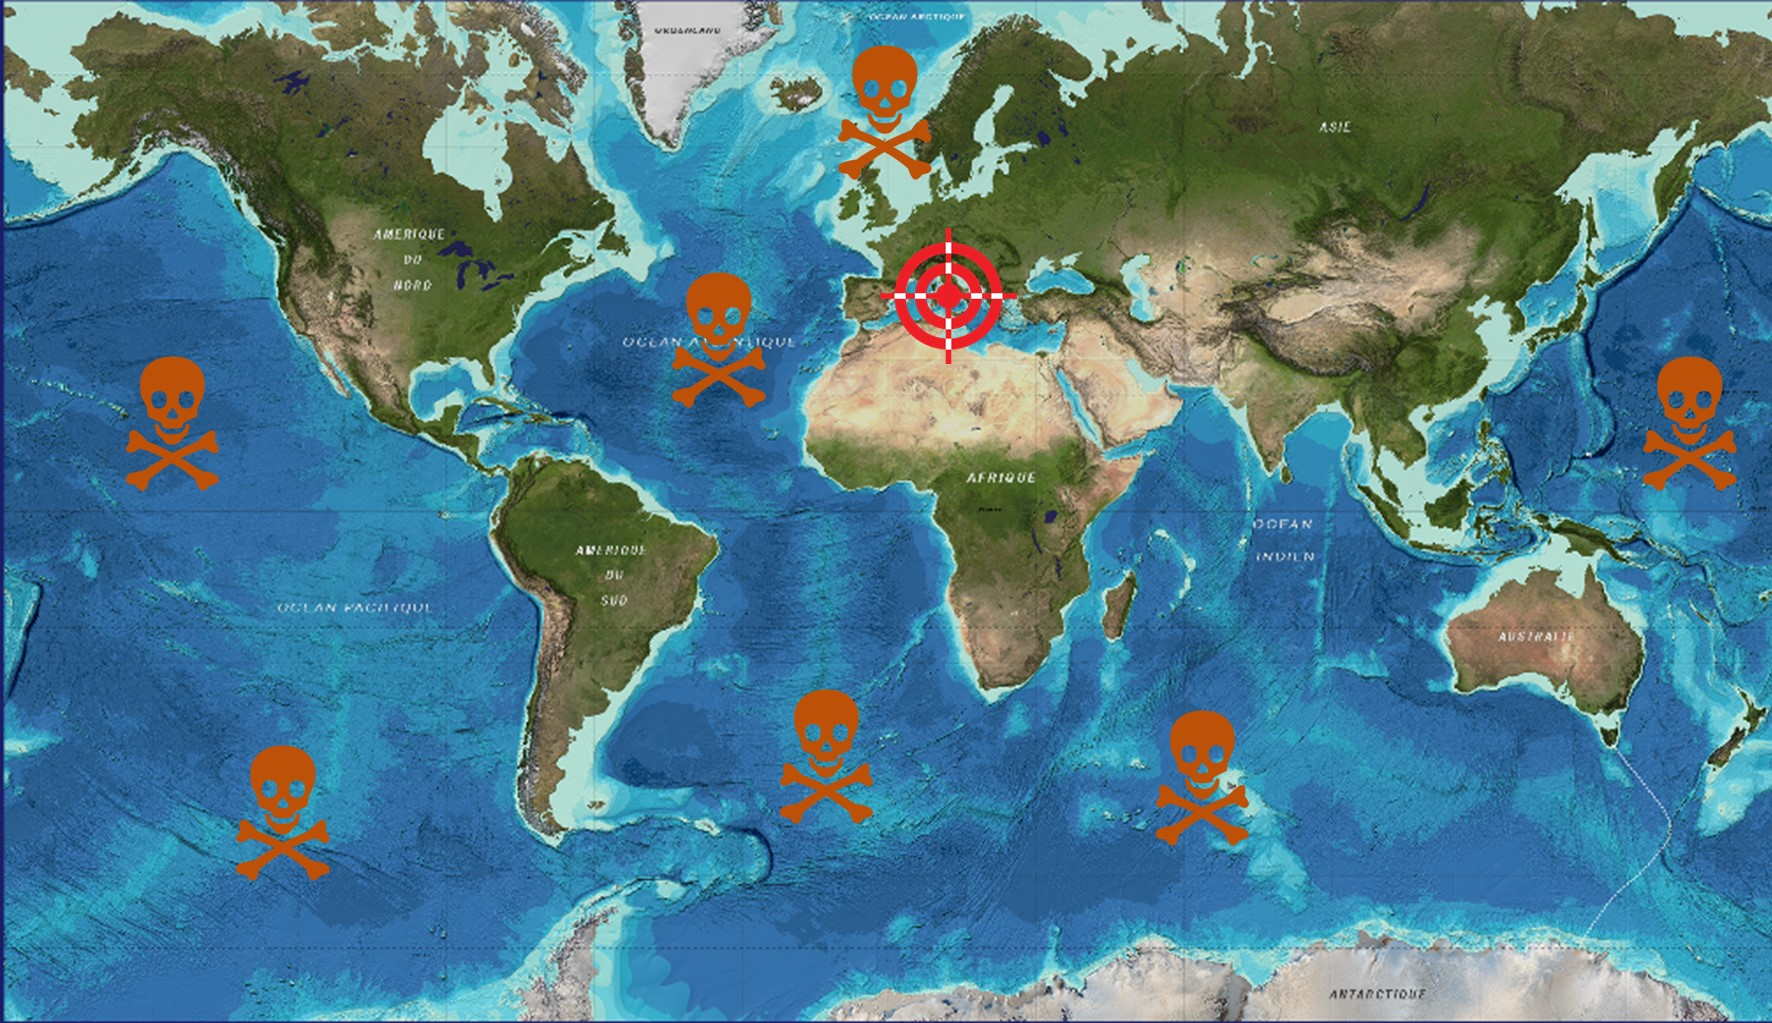
\includegraphics[width=\linewidth,keepaspectratio]{./1_intro/cover_intro}}
 \node [inner sep=0pt](mypicture) at (0,0) {\phantom{\ig}};
 \clip[rounded corners=5mm] ($(mypicture.south west)+(\bord,\bord)$) rectangle ($(mypicture.north east)-(\bord,\bord)$);
 \node[inner sep=0pt](mypicture) at (0,0) {\ig};
\end{tikzpicture}


% Table des matières intro
{\LARGE
\begin{enumerate}[label=\textcolor{bleusection}{\arabic*}{.}, leftmargin=2cm]
  \item \nameref{intro.1}
  \item \nameref{intro.2}
  \item \nameref{intro.3}
\end{enumerate}
}

% DEBUT INTRO
\clearpage
\pagestyle{intro}


\section{Une biodiversité marine en danger}\label{intro.1}

\subsection{Distribution de la biodiversité marine mondiale}\label{intro.1.1}

Les océans couvrent plus de 70 \% de la surface de la Terre, abritent 50 à 80 \% des espèces vivantes de notre planète \citep{mora_how_2011, costello_global_2013}, et génèrent plus de 60 \% des services écosystémiques mondiaux \citep{millenium_ecosystem_assessment_ecosystem_2005, bindoff_changing_2019, ipbes_global_2019}, dont la moitié de la production du dioxygène atmosphérique par photosynthèse. L’océan global est un organe clé de la régulation du système climatique, via les flux thermiques et biogéochimiques qu’il entretient avec l’atmosphère ; il est notamment responsable de l’absorption de plus de 25 \% des émissions annuelles de CO\textsubscript{2} d’origine anthropique \citep{heinze_ocean_2015}.

L’étendue géographique de l’océan global, du pôle Sud au pôle Nord, ainsi que sa très forte anisotropie verticale (notamment température et lumière) créent de nombreuses niches écologiques, peu à peu exploitées au cours de l’évolution par une grande diversité de formes vivantes. Si la répartition de la biodiversité océanique mondiale dépend du taxon considéré, elle est plus importante en milieu côtier \citep{tittensor_global_2010}, et particulièrement forte en milieu tropical, notamment dans le « triangle de corail » \citep{sanciangco_habitat_2013} (Malaisie, Indonésie, Philippines et îles Salomon ; \autoref{figure_intro1}).

%%%%%%%%%%%%%%%%%%%%%%%%%%%%%%%%%%%%%%%%%%%%%%%%%%%%%%%%%%%%%
%%% Figure intro1: Cartographie de la richesse spécifique %%%
%%%%%%%%%%%%%%%%%%%%%%%%%%%%%%%%%%%%%%%%%%%%%%%%%%%%%%%%%%%%%
\begin{figure}[H]
	\begin{center}
	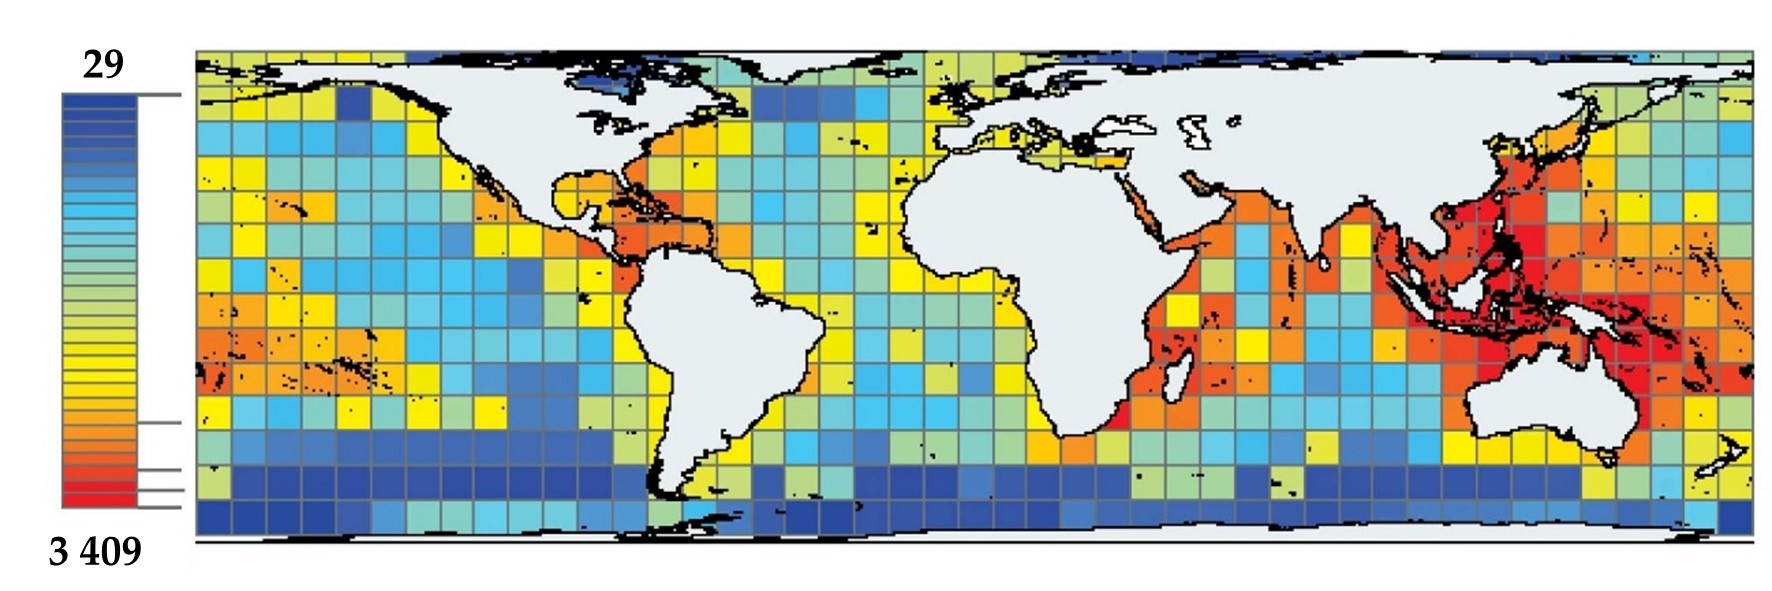
\includegraphics[width=\linewidth,keepaspectratio]{./1_intro/global_diversity_Tittensor2010}
		\caption[Cartographie de la richesse spécifique mondiale tous taxa confondus]{Cartographie de la richesse spécifique mondiale tous taxa confondus (d'après \citet{tittensor_global_2010}). Données compilées pour 11 567 espèces appartenant à 13 taxa différents.}
	\label{figure_intro1}
\end{center}
\end{figure}

\subsection{Une biodiversité sous pression}\label{intro.1.2}

\subsubsection{Contexte de changement global}\label{intro.1.2.1}
La compréhension de la distribution des espèces ainsi que des forces structurant les assemblages ont toujours intéressé les biologistes depuis les premiers travaux de Darwin \citep{darwin_origin_1859}. La prise en compte des impacts anthropiques sur la biodiversité mondiale et l’urgence de mettre en place des plans de conservation efficaces pour sa préservation \citep{margules_systematic_2000} ont motivé la poursuite des études sur les patrons de biodiversité à différentes échelles spatiales \citep{rosa_multiscale_2017}. En effet, la très forte intensification des émissions de gaz à effet de serre depuis le début de l’ère industrielle a déjà contribué à d’importantes perturbations du système climatique à toutes les échelles spatiales, et les projections indiquent une poursuite de ces modifications climatiques pour les décennies à venir \citep{ipcc_climate_2013}. Cette altération du climat, associée aux autres pressions anthropiques (déforestation, surpêche, pollutions chimiques…), a déjà largement affecté la biosphère au point d’initier la « sixième crise d’extinction d’espèces » \citep{barnosky_has_2011, dirzo_defaunation_2014, ceballos_accelerated_2015}. Tous les scénarii indiquent que cette érosion de la biodiversité devrait se poursuivre au cours du 21e siècle \citep{pereira_scenarios_2010, tittensor_mid-term_2014, visconti_projecting_2016}.

Les océans ne sont pas indemnes des impacts de « l’Anthropocène » \citep{mcgill_fifteen_2015}, et l’érosion de la biodiversité marine continue de s’accélérer \citep{mccauley_marine_2015, bindoff_changing_2019, ohara_mapping_2019}. En effet, la température est le principal facteur environnemental régissant la distribution des espèces marines \citep{tittensor_global_2010}, et les modifications de la température des océans questionnent sur une possible redistribution des espèces et des assemblages écologiques à l’échelle globale \citep{pereira_scenarios_2010, tittensor_global_2010, poloczanska_responses_2016}. Les habitats marins côtiers sont particulièrement vulnérables dans la mesure où ils abritent une importante biodiversité \citep{halpern_global_2008} et sont directement soumis à une population humaine beaucoup plus dense que la moyenne (27 \% de la population mondiale vit à moins de 100 km de la côte \citep{kummu_over_2016}). Parmi eux, les récifs coralliens sont largement étudiés, car ils contiennent à eux seuls environ 35 \% de la biodiversité marine mondiale \citep{reaka-kudla_biodiversity_2005} et sont largement touchés par le changement climatique \citep{hoegh-guldberg_coral_2007, death_27-year_2012, graham_predicting_2015, hughes_coral_2017}. Bien que certains assemblages tempérés semblent plus robustes que les récifs coralliens tropicaux aux changements globaux \citep{stuart-smith_stability_2010}, la majorité des biomes marins sont susceptibles d’être affectés \citep{waycott_accelerating_2009, marba_mediterranean_2014, telesca_seagrass_2015, wernberg_climate-driven_2016, halpern_recent_2019, ohara_mapping_2019}. Les résultats plus mitigés en milieu tempéré pourraient être en partie expliqués par un manque de données pour ces habitats \citep{wernberg_impacts_2011}. En effet, la situation en 2008 indiquait que plus de 40 \% des océans subissaient déjà un fort impact anthropique cumulé \citep{halpern_global_2008}, et cet impact a significativement augmenté au cours de la dernière décennie pour près de 60 \% des océans \citep{halpern_recent_2019} (\autoref{figure_intro2}). Aujourd’hui, près de la totalité de l’océan mondial (97,7 \%) est affectée par plusieurs pressions anthropiques \citep{halpern_spatial_2015} et 83 \% de l’océan global abrite plus de 25 \% d’espèces menacées \citep{ohara_mapping_2019}.

%%%%%%%%%%%%%%%%%%%%%%%%%%%%%%%%%%%%%%%%%%%%%%%%%%%
%%% Figure intro2: Cartographie impacts cumulés %%%
%%%%%%%%%%%%%%%%%%%%%%%%%%%%%%%%%%%%%%%%%%%%%%%%%%%
\begin{figure}[H]
	\begin{center}
	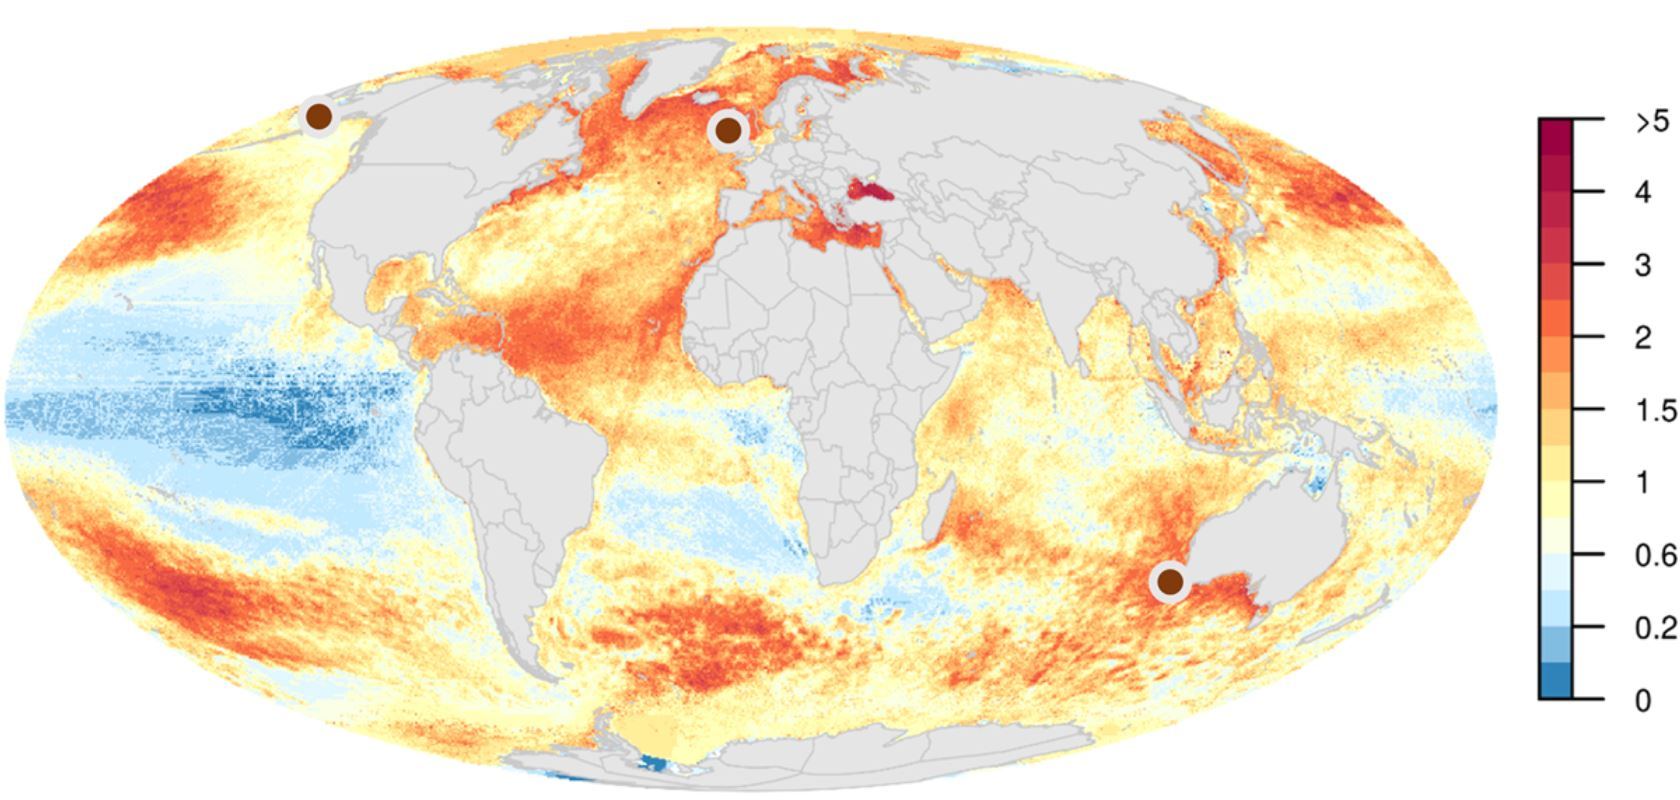
\includegraphics[width=\linewidth,keepaspectratio]{./1_intro/cumulative_impacts_Halpern2019}
		\caption[Cartographie des impacts anthropiques cumulés à l’échelle mondiale]{Cartographie des impacts anthropiques cumulés à l’échelle mondiale (d'après \citet{halpern_recent_2019}).}
	\label{figure_intro2}
\end{center}
\end{figure}

\subsubsection{Pressions anthropiques locales}\label{intro.1.2.2}
Les changements globaux induits par les émissions massives de gaz à effet de serre depuis le début de l’ère industrielle ne sont malheureusement pas les seuls facteurs affectant la biodiversité, et les écosystèmes sont menacés à l’échelle globale par de multiples pressions anthropiques \citep{hoekstra_confronting_2004, halpern_global_2008}. Par exemple, la fragmentation et la perte d’habitats ont des effets considérables sur leur biodiversité \citep{brooks_habitat_2002, haddad_habitat_2015}. Les habitats marins, bien qu’en apparence protégés de l’action de l’Homme, subissent d’importantes pressions anthropiques locales \citep{micheli_cumulative_2013, halpern_spatial_2015, holon_predictive_2018} (\autoref{figure_intro3}), avec notamment : \textbf{la pêche} (dégradation des habitats par chalutage \citep{hiddink_global_2017}, effondrement des stocks halieutiques à cause de la surpêche \citep{christensen_century_2014, essington_fishing_2015, link_global_2019} et impacts des engins de pêche laissés à l’abandon \citep{wilcox_understanding_2015, moschino_is_2019}), \textbf{les aménagements côtiers} (destruction des habitats et perturbation des régimes hydrosédimentaires favorisant la sédimentation sur des habitats sensibles \citep{airoldi_effects_2003, holon_predictive_2018}), \textbf{les pratiques agricoles} (enrichissement en nitrates et phosphates modifiant la structure des communautés \citep{berger_effects_2003, savage_effects_2010}), \textbf{les rejets de station d’épuration} (pathogènes, matière organique et nutriments altèrent la qualité de l’eau et affectent les habitats limitrophes \citep{orth_global_2006, waycott_accelerating_2009}), \textbf{le trafic maritime} (collisions avec les cétacés \citep{peltier_monitoring_2019}, perturbation des vertébrés marins \citep{bruintjes_rapid_2016, simpson_anthropogenic_2016, bas_marine_2017,slabbekoorn_effects_2018}), \textbf{le mouillage} (dégradation des herbiers sous-marins \citep{short_natural_1996} et des récifs biogéniques \citep{ballesteros_mediterranean_2006} par l’action mécanique de l’ancre et de la chaîne \citep{milazzo_boat_2004}), \textbf{les espèces exotiques envahissantes} (une des principales causes d’extinction d’espèces \citep{bellard_alien_2016}, considérée comme l’un des plus grands défis en matière de conservation \citep{pysek_invasive_2010}), et \textbf{les rejets de macro-déchets plastiques} (chaque année, plus de 300 millions de tonnes de déchets plastiques atterrissent dans l’océan global \citep{law_plastics_2017} et contaminent un nombre significatif d’espèces marines les ingérant \citep{schuyler_global_2013, wilcox_threat_2015}).

%%%%%%%%%%%%%%%%%%%%%%%%%%%%%%%%%%%%%%%%%%%%%%%%%%%%%%%%%%
%%% Figure intro3: Illustration pressions anthropiques %%%
%%%%%%%%%%%%%%%%%%%%%%%%%%%%%%%%%%%%%%%%%%%%%%%%%%%%%%%%%%
\begin{figure}[H]
	\begin{center}
	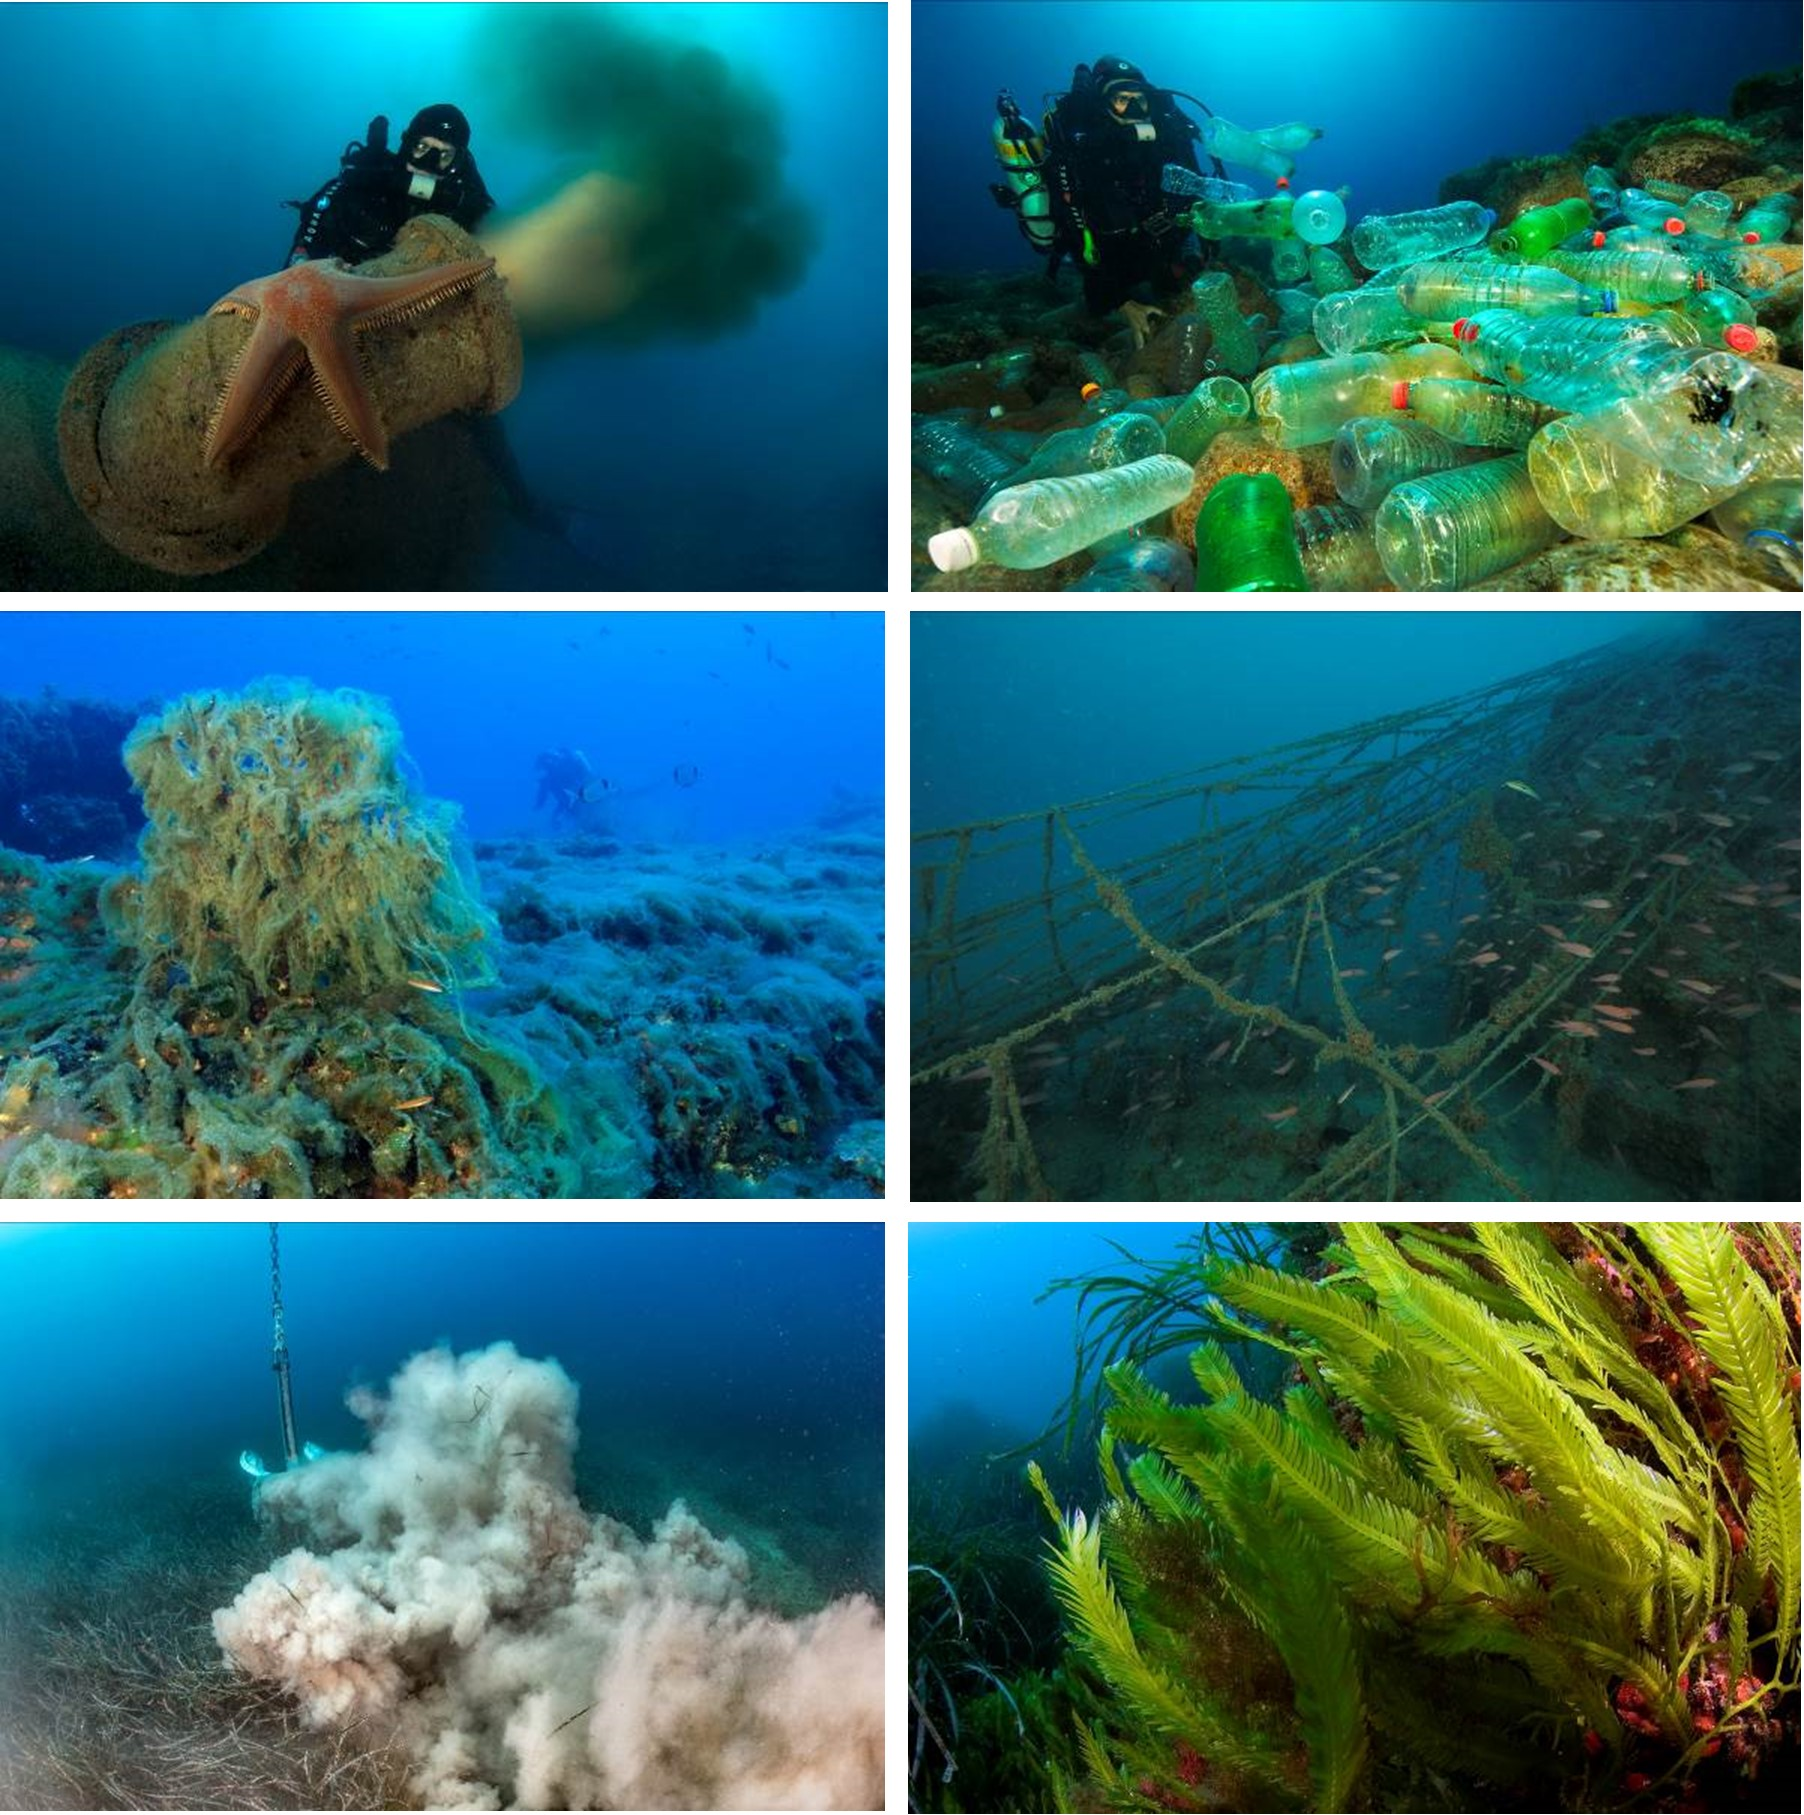
\includegraphics[width=\linewidth,keepaspectratio]{./1_intro/pressions}
		\caption[Illustrations de quelques pressions anthropiques]{Illustrations de quelques pressions anthropiques. De gauche à droite et de haut en bas: rejet de station d’épuration, macro-déchets plastiques, algues filamenteuses recouvrant un récif coralligène et ses gorgones, ancien engin de pêche coincé sur un récif coralligène, relève d’une ancre d’un bateau au mouillage dans l’herbier, présence d’une espèce exotique envahissante (\textit{Caulerpa taxifolia}) dans un herbier de posidonie (\textit{©Andromède Océanologie}).}
	\label{figure_intro3}
\end{center}
\end{figure}

\subsection[La Méditerranée: une exceptionelle biodiversité soumise à d’importantes pressions]{La Méditerranée: une exceptionelle biodiversité soumise à \\ d’importantes pressions}\label{intro.1.3}

Située entre l’Europe et l’Afrique, la mer Méditerranée est ce qu’il reste aujourd’hui de l’océan Téthys. Son histoire géologique intense, sa géomorphologie et ses conditions environnementales ont largement contribué à son histoire évolutive et à l’exceptionnelle biodiversité qui la caractérise depuis la fin de l’Éocène (-42 Ma à -39 Ma) \citep{boudouresque_marine_2004, renema_hopping_2008}. Aujourd’hui, alors qu’elle ne représente que 0,32 \% du volume de l’océan global, la mer Méditerranée abrite près de 7 \% de la biodiversité marine mondiale (17 000 espèces) \citep{coll_biodiversity_2010} dont environ un quart est endémique au bassin \citep{bianchi_rmesualtrsine_2000}. L’essentiel de cette biodiversité se concentre sur le plateau continental, notamment les poissons et les invertébrés benthiques (vivant sur le fond) \citep{coll_mediterranean_2012, katsanevakis_invading_2014} (\autoref{figure_intro4}). L’exploitation des ressources halieutiques a été un facteur primordial dans l’établissement et le développement des civilisations autour du bassin Méditerranéen au cours de l’histoire \citep{coll_biodiversity_2010}, mais représente aujourd’hui une menace pour cette biodiversité côtière. Par ailleurs, la Méditerranée n’est pas épargnée par les changements climatiques et représente une des régions les plus vulnérables aux perturbations climatiques futures \citep{giorgi_climate_2006, adloff_mediterranean_2015}. Les herbiers de posidonie (Posidonia oceanica) et les récifs coralligènes, qui figurent parmi les habitats marins les plus riches de Méditerranée \citep{boudouresque_marine_2004}, sont particulièrement sujets aux fortes pressions anthropiques globales et locales. 

%%%%%%%%%%%%%%%%%%%%%%%%%%%%%%%%%%%%%%%%%%%%%%%%%%%%%%%
%%% Figure intro4: Richesse spécifique Méditerranée %%%
%%%%%%%%%%%%%%%%%%%%%%%%%%%%%%%%%%%%%%%%%%%%%%%%%%%%%%%
\begin{figure}[H]
	\begin{center}
	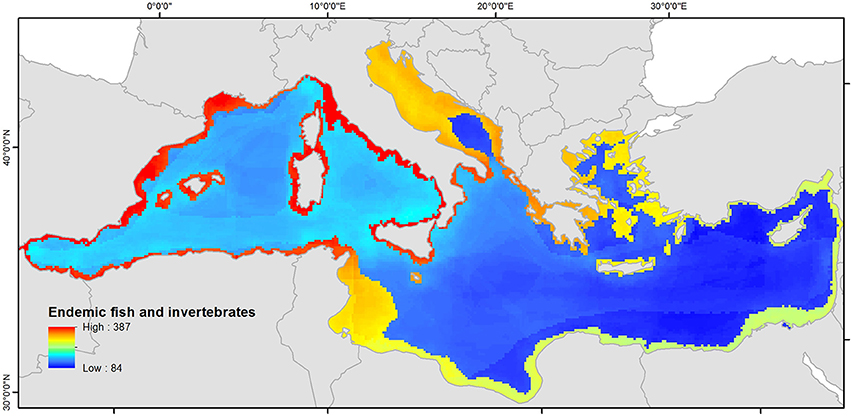
\includegraphics[width=\linewidth,keepaspectratio]{./1_intro/species_richness_Katsanevakis2014}
		\caption[Richesse spécifique des poissons et invertébrés endémiques en Méditerranée]{Richesse spécifique des poissons et invertébrés endémiques en Méditerranée \citep{katsanevakis_invading_2014}.}
	\label{figure_intro4}
\end{center}
\end{figure}

\subsubsection{Les herbiers de Posidonie : un habitat fragile aux multiples services écosystémiques}\label{intro.1.3.1}

La notion de services écosystémiques vise à quantifier l’ensemble des bénéfices que les humains tirent du fonctionnement et de l’intégrité des écosystèmes \citep{de_groot_global_2012}. Si les services attribués aux écosystèmes marins sont encore peu documentés \citep{townsend_challenge_2018}, plus de la moitié de la valeur du capital naturel et des services écosystémiques mondiaux sont attribués aux seuls herbiers sous-marins \citep{millenium_ecosystem_assessment_ecosystem_2005, ipbes_global_2019}. En effet, leurs rôles écologiques et économiques sont cruciaux : séquestration de carbone dans les rhizomes et la matte, production primaire locale pour les herbivores, export de matière organique vers les habitats à faible production, oxygénation de la colonne d’eau, atténuation de la houle, fixation du sédiment et des matières en suspension, nurserie à poissons… (\autoref{figure_intro5}).

%%%%%%%%%%%%%%%%%%%%%%%%%%%%%%%%%%%%%%%%%%%%%%%%%%%%%%%
%%% Figure intro5: Richesse spécifique Méditerranée %%%
%%%%%%%%%%%%%%%%%%%%%%%%%%%%%%%%%%%%%%%%%%%%%%%%%%%%%%%
\begin{figure}[H]
	\begin{center}
	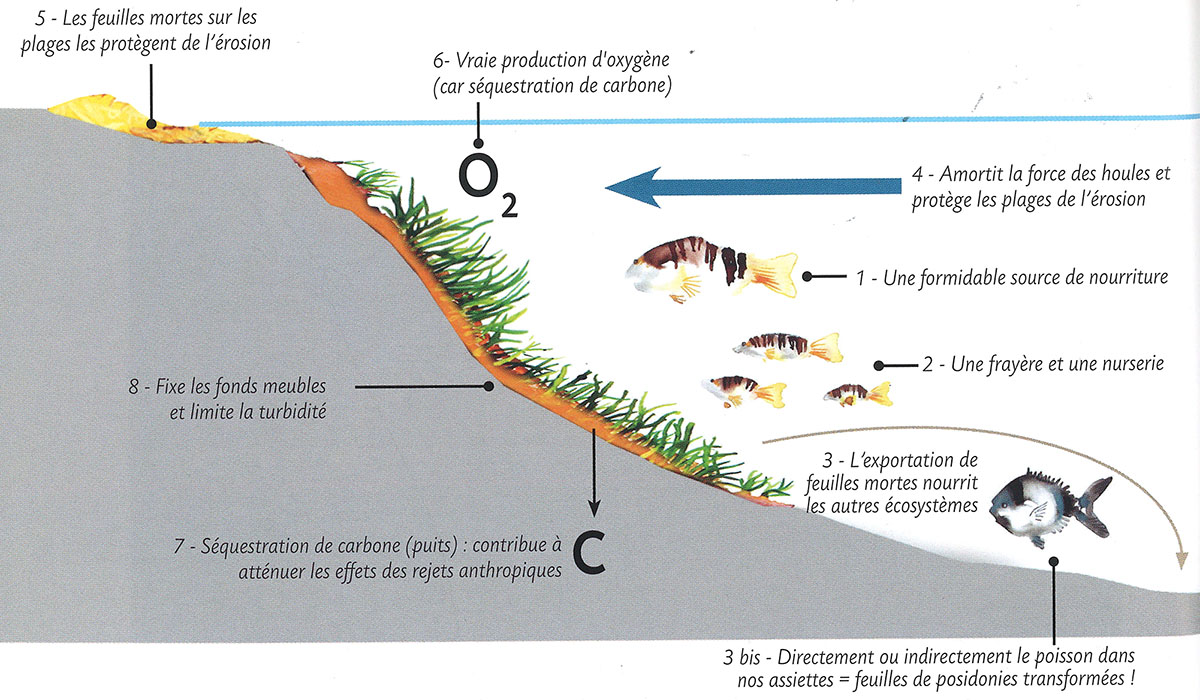
\includegraphics[width=\linewidth,keepaspectratio]{./1_intro/services_herbiers_posidonies_Boudouresque}
		\caption[Services écosystémiques fournis par les herbiers sous-marins]{Services écosystémiques fournis par les herbiers sous-marins (source : \href{https://planet-vie.ens.fr}{https://planet-vie.ens.fr}).}
	\label{figure_intro5}
\end{center}
\end{figure}

La posidonie (\textit{Posidonia oceanica}), une espèce protégée endémique de Méditerranée, forme de grandes prairies sous-marines entre la surface et 40 m de fond (\autoref{figure_intro6}). En raison de sa proximité à la côte et à la surface, cette espèce souffre tout particulièrement des effets des changements globaux \citep{marba_mediterranean_2014} et des pressions locales telles que l’augmentation de la population et de l’urbanisation côtières, responsables de la destruction et de la dégradation de cet habitat fragile \citep{montefalcone_human_2010, marba_mediterranean_2014, holon_impact_2015, telesca_seagrass_2015}. Les herbiers de posidonie sont reconnus comme un « habitat d’intérêt spécifique » en termes de biodiversité par la directive européenne concernant la conservation des habitats naturels ainsi que de la faune et de la flore sauvages (Directive Habitats 92/43/CEE).

%%%%%%%%%%%%%%%%%%%%%%%%%%%%%%%%%%%%%%%%%%%%%%%%%%%%%%%%%%
%%% Figure intro6: Illustrations herbiers de posidonie %%%
%%%%%%%%%%%%%%%%%%%%%%%%%%%%%%%%%%%%%%%%%%%%%%%%%%%%%%%%%%
\begin{figure}[H]
	\begin{center}
	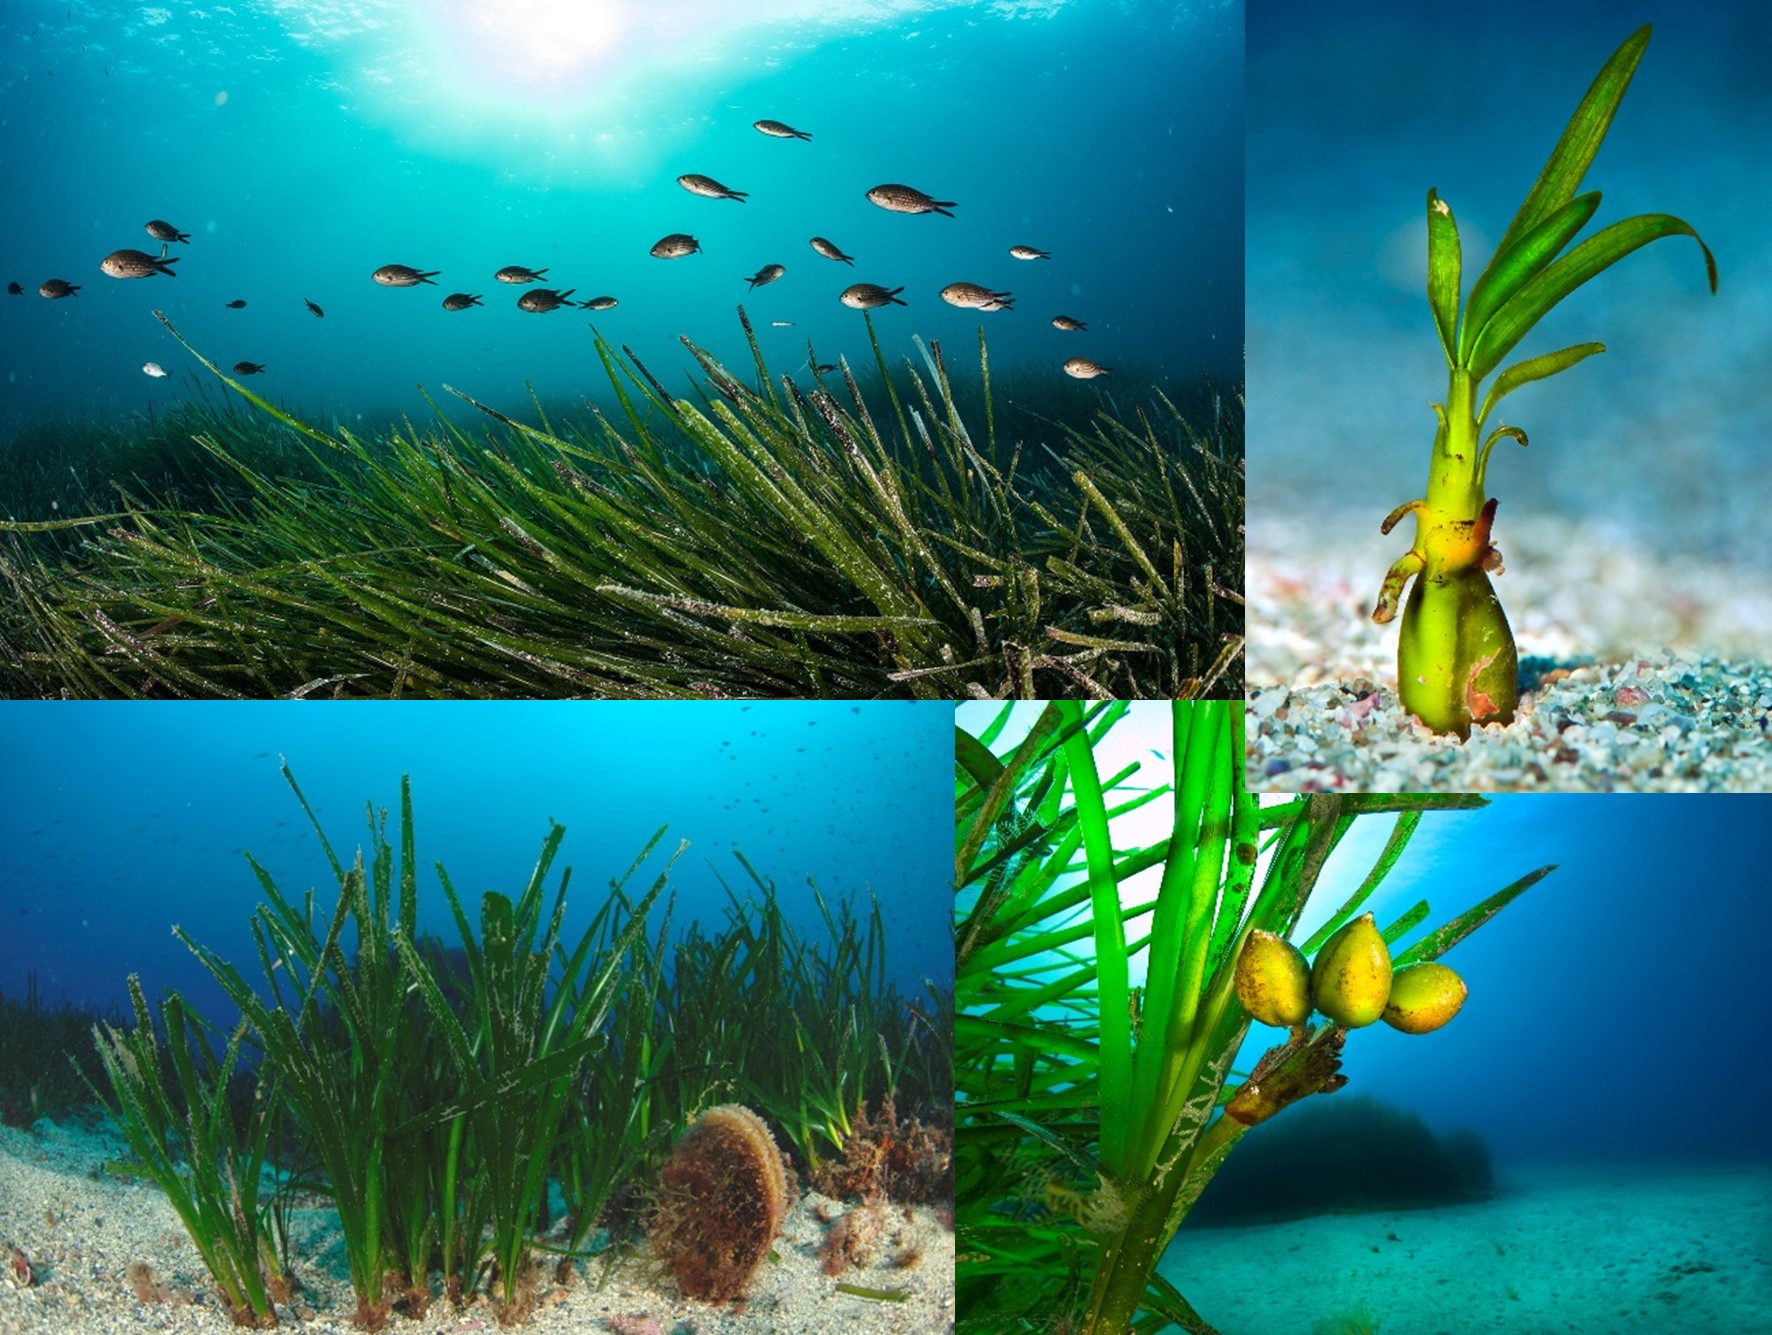
\includegraphics[width=\linewidth,keepaspectratio]{./1_intro/herbiers_posidonie}
		\caption[Illustrations d’un herbier de Posidonie]{Illustrations d’un herbier de Posidonie. De haut en bas et de gauche à droite : herbier avec quelques castagnoles (\textit{Chromis chromis}) ; graine germée de posidonie ; herbier avec une grande nacre (\textit{Pinna nobilis}) ; plant de posidonie avec ses graines) (\textit{©Andromède Océanologie}.}
	\label{figure_intro6}
\end{center}
\end{figure}

\subsubsection{Les récifs coralligènes : une biodiversité semblable aux récifs coralliens}\label{intro.1.3.2}

Les récifs coralligènes sont produits par l’accumulation de plus de 1500 espèces d’algues calcaires encroûtantes et d’animaux bioconstructeurs (polychètes, bryozoaires et gorgonaires) \citep{ballesteros_mediterranean_2006}; ce sont les seules formations calcaires d’origine biogénique en Méditerranée \citep{ballesteros_mediterranean_2006}, et leur diversité et productivité sont similaires à celles des récifs coralliens \citep{bianchi_biocostruzione_2001}. Ces récifs sont des niches écologiques importantes pour un grand nombre d’espèces mobiles : poissons, crustacés, échinodermes, mollusques, tuniqués \citep{ballesteros_mediterranean_2006} (\autoref{figure_intro7}). Comme les herbiers de posidonie, l’habitat « récifs coralligènes » est reconnu comme « habitat d’intérêt spécifique » en termes de biodiversité par la directive européenne concernant la conservation des habitats naturels ainsi que de la faune et de la flore sauvages (Directive Habitats 92/43/CEE).

%%%%%%%%%%%%%%%%%%%%%%%%%%%%%%%%%%%%%%%%%%%%%%%%%%%%%%%%
%%% Figure intro7: Illustrations récifs coralligènes %%%
%%%%%%%%%%%%%%%%%%%%%%%%%%%%%%%%%%%%%%%%%%%%%%%%%%%%%%%%
\begin{figure}[H]
	\begin{center}
	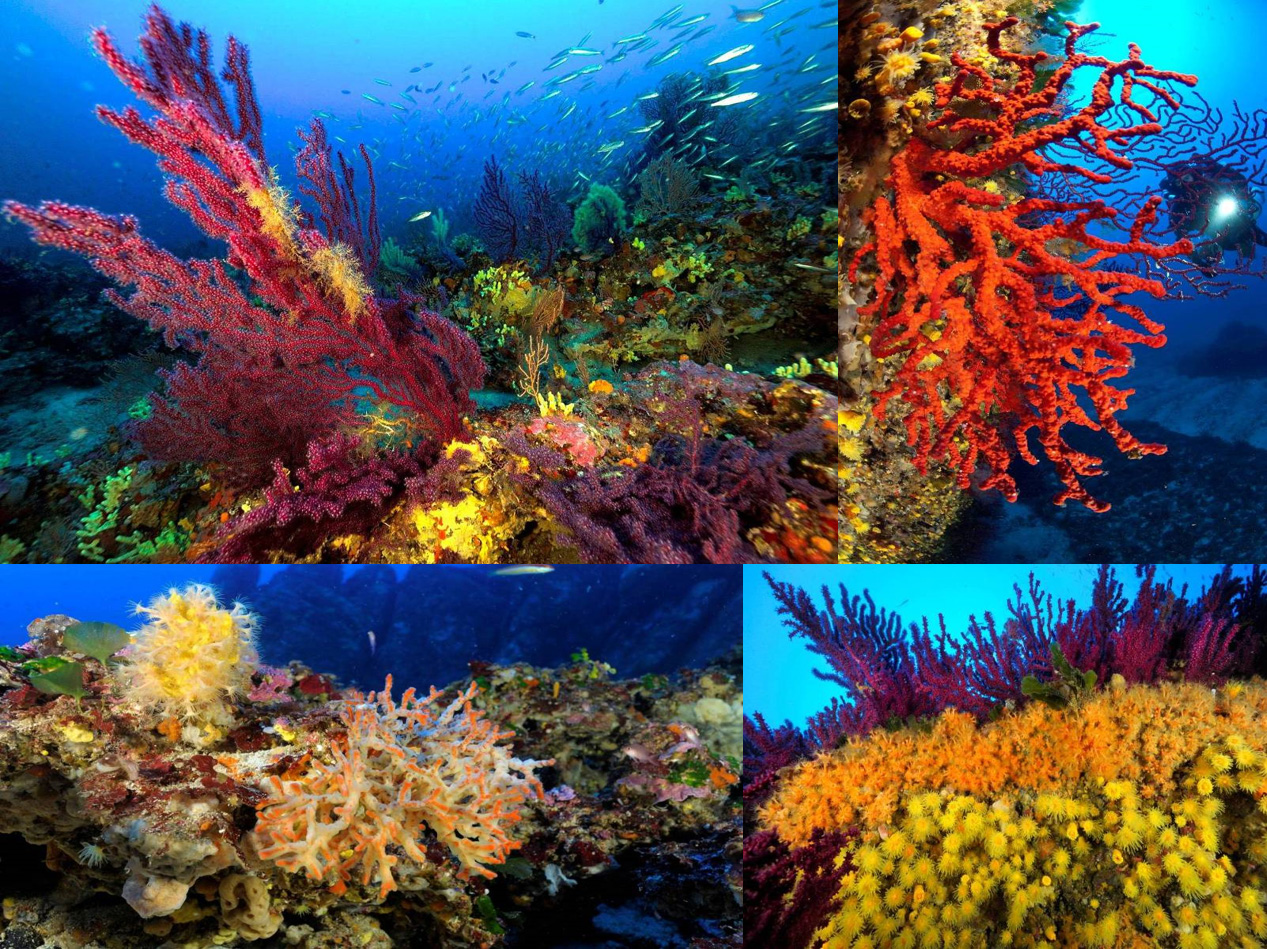
\includegraphics[width=\linewidth,keepaspectratio]{./1_intro/recifs_coralligenes}
		\caption[Illustrations des assemblages des récifs coralligènes]{Illustrations des assemblages des récifs coralligènes (\textit{©Andromède Océanologie}).}
	\label{figure_intro7}
\end{center}
\end{figure}

Bien que situés à des profondeurs allant de 12 à 120 m \citep{ballesteros_mediterranean_2006}, les récifs coralligènes ne sont pas exempts des effets des multiples pressions anthropiques qui affectent la biodiversité marine. Cet habitat est particulièrement affecté par l’accroissement de la sédimentation provoquée par les activités anthropiques côtières et les modifications de régimes hydro-sédimentaires \citep{airoldi_effects_2003}, ainsi que par la pêche et le mouillage \citep{ballesteros_mediterranean_2006}. 

\medskip

\setlength{\fboxsep}{5pt}
\setlength{\fboxrule}{0.6pt}
\noindent\framebox{%
  \begin{minipage}{\linewidth}
    La \textbf{biodiversité marine} est d’une \textbf{exceptionnelle richesse}, et l’humanité entière dépend des nombreux \textbf{services écosystémiques} qu’elle fournit. Pourtant, de nombreuses pressions anthropiques attaquent et érodent cette biodiversité, notamment en milieu côtier, où les densités de populations humaines et la biodiversité sont les plus élevées. \textbf{La Méditerranée} est le parfait exemple de cette co-occurrence de hauts niveaux de biodiversité et de pression, dans un espace géographique semi-fermé et restreint. La mise en place de \textbf{moyens de conservation efficaces} pour \textbf{préserver les écosystèmes marins} est aujourd’hui cruciale, mais la méconnaissance de ce milieu limite les actions visant à réduire son altération. Il est donc indispensable de \textbf{mettre en place des réseaux de surveillance} afin d’étudier et suivre l’état de santé des habitats marins, pour anticiper les changements et \textbf{assister les décisionnaires} dans la gestion de ces habitats.
  \end{minipage}}

\newpage

\section{Surveillance de la biodiversité marine}\label{intro.2}

Compte tenu de la crise climatique actuelle et de la sensibilité des assemblages marins aux diverses pressions anthropiques, il est nécessaire d’étudier et de suivre les dynamiques spatio-temporelles de la biodiversité marine afin de mettre en place des mesures de conservation efficaces \citep{magris_integrating_2014, klein_shortfalls_2015}. La surveillance globale de la biodiversité et de son évolution, notamment face aux changements climatiques, nécessite de s’accorder sur les \textbf{variables essentielles pour la biodiversité} (« Essential Biodiversity Variables », EBVs) à mesurer pour quantifier ces changements \citep{pereira_essential_2013, navarro_monitoring_2017, schmeller_operational_2017, haase_next_2018, kissling_building_2018}. L’intérêt de la conceptualisation des EBVs est né d’un besoin de structurer et d’harmoniser les données relatives à la surveillance de la biodiversité à différentes échelles spatiales et temporelles \citep{kissling_building_2018} afin de répondre aux objectifs de la Convention sur la Diversité Biologique (CDB 2010). Aujourd’hui, ces EBVs et les indicateurs qui en découlent doivent permettre de répondre aux besoins essentiels de la biodiversité dans le cadre de l’Agenda 2030 et ses objectifs de développement durable (Biodiversity and the 2030 Agenda for Sustainable Development). Elles constituent un premier niveau d’abstraction entre les \textbf{observations brutes} et les \textbf{indicateurs de biodiversité} ; on en distingue six classes : composition génétique, dynamique et distribution de populations, traits spécifiques, composition des communautés, fonctionnement et structure de l’écosystème \citep{pereira_essential_2013}. Dans le cadre de ce travail doctoral, nous nous concentrerons essentiellement sur la \textbf{distribution de populations}, la \textbf{composition des communautés} et la \textbf{structure de l’écosystème}.

\subsection{Indicateurs de biodiversité}\label{intro.2.1}

Si fondamentalement, elle cherche à caractériser la richesse biologique de notre planète, la notion de « biodiversité » semble bien complexe et protéiforme. En effet, elle inclut différentes échelles et différentes mesures quantitatives et qualitatives, il est donc extrêmement difficile de l’exprimer avec une seule métrique, et de très nombreux indices ont été développés \citep{teixeira_catalogue_2016}. Dans ce manuscrit, nous nous intéresserons à des indicateurs communs d’évaluation des assemblages écologiques ainsi qu’à des indicateurs originaux visant à décrire la structure de l’habitat. Plus particulièrement, nous utiliserons les indicateurs suivants pour caractériser les habitats marins :

\begin{itemize}
    \item \textbf{Diversité taxonomique} (ou « richesse spécifique ») : mesure la plus simple de la biodiversité, elle correspond au nombre d’espèces différentes observées dans un espace donné et à un moment donné. Ce nombre n’a jamais vocation à être exhaustif, et se limite souvent à ce qui est facilement observable (ex. : la diversité bactérienne est plus difficile à mesurer que la diversité d’oiseaux) ;
    
    \item \textbf{Indice de Shannon} \citep{magurran_measuring_2004} : semblable à la diversité taxonomique, il dépend non seulement du nombre d’espèces différentes observées, mais également de leur abondance relative. En effet, il convient de pouvoir distinguer deux communautés composées des mêmes espèces mais dont l’une aurait des abondances équitablement réparties entre espèces, et l’autre dominée par une ou plusieurs espèces. Cet indicateur reprend la forme de l’entropie, il est calculé comme suit :
    
    \begin{equation}
	    S_j=-\sum_{i}p_{ij} log(p_{ij})
	    \label{eqintro.1}
    \end{equation}
    
    Avec \textit{p\textsubscript{ij}} la prévalence de l’espèce $i$ au sein du site $j$.
    
    \item \textbf{Diversité fonctionnelle} : toutes les espèces présentent des caractéristiques morphologiques (taille, forme, biomasse…) et comportementales (relations trophiques, mode de reproduction, mobilité, migrations…) très différentes et parfois uniques, appelées « traits fonctionnels ». De fait, les espèces ne sont fonctionnellement pas équivalentes et il convient de pouvoir distinguer des assemblages en prenant en compte cette diversité, essentielle au bon fonctionnement des écosystèmes et à la provision de services écosystémiques dont dépendent les humains \citep{hooper_effects_2005, cadotte_using_2009, clemente_identifying_2010, faith_evosystem_2010}. Une multitude d’indices ont été développés afin de quantifier cette diversité fonctionnelle \citep{petchey_functional_2002, magurran_measuring_2004, mouchet_towards_2008, villeger_new_2008}~;
    
    \item \textbf{Structure de l’habitat} : si ses effets sur la biodiversité ne sont pas systématiquement négatifs (Fahrig, 2017), la \textbf{fragmentation} des habitats est connue pour jouer un rôle important dans la structuration et la dynamique des assemblages écologiques \citep{wilson_habitat_2016, crooks_quantification_2017}. La fragmentation peut se mesurer avec différents indicateurs paysagers \citep{de_montis_landscape_2017}. Par ailleurs, de nombreuses études ont montré que la \textbf{complexité structurale} de l’habitat avait un effet important sur la structuration des communautés, notamment l’abondance et la diversité des espèces marines \citep{luckhurst_analysis_1978, gratwicke_relationship_2005, harborne_biotic_2011, meager_topographic_2011, kovalenko_habitat_2012, graham_importance_2013, rees_abiotic_2014, darling_relationships_2017}. La complexité structurale se mesure généralement grâce à la \textbf{rugosité} de l’habitat \citep{friedman_multi-scale_2012, dustan_digital_2013, leon_measuring_2015} ou à sa \textbf{dimension fractale} \citep{yanovski_structural_2017, young_cost_2017, fukunaga_integrating_2019}.
    
\end{itemize}

\setlength{\fboxsep}{5pt}
\setlength{\fboxrule}{0.6pt}
\noindent\framebox{%
  \begin{minipage}{\linewidth}
    La \textbf{biodiversité} est une notion complexe \underline{qu’on ne peut pas synthétiser en un seul indicateur}. Dans le cas de \textbf{suivis écologiques} et l’étude des assemblages, il convient de mesurer différents compartiments et \textbf{calculer différents indicateurs} pour fournir une évaluation satisfaisante de \textbf{l’état d’un écosystème} et de son \textbf{fonctionnement}.
  \end{minipage}
}

\subsection[Méthodes d’acquisition d’images et de données cartographiques marines]{Méthodes d’acquisition d’images et de données \\cartographiques marines}\label{intro.2.2}

Afin d’évaluer la biodiversité marine et de quantifier les effets des pressions anthropiques, il est indispensable de \textbf{cartographier la présence} des espèces marines et de \textbf{quantifier leur abondance} à différentes échelles (principe des EBVs de distribution de populations) :

\begin{itemize}
    \item \textbf{Inventaires à méso/macro-échelle} avec une \underline{longue période de retour} pour étudier les facteurs environnementaux régissant la \underline{distribution des espèces}, et quantifier à plus large échelle les effets des pressions anthropiques ;
    
    \item \textbf{Inventaires à micro-échelle} avec une \underline{courte période de retour} pour comprendre la\\ \underline{complexité des assemblages} de certains habitats et détecter localement des changements précoces dans les équilibres écologiques.
\end{itemize}

Ces inventaires sont réalisés à l’aide de différentes méthodes d’acquisition, notamment des méthodes d’acquisition d’images qui permettent de déterminer la nature des assemblages et de cartographier l’étendue géographique des espèces. Si la colonne d’eau représente une forte contrainte pour l’étude des habitats marins, elle stimule le développement de méthodes cartographiques innovantes. Parmi elles, il convient de distinguer les méthodes cartographiques à méso/macro-échelle par télédétection, et à micro-échelle par proxy-détection et mesures \textit{in situ}.

\subsubsection{Cartographie à méso/macro-échelle par télédétection}\label{intro.2.2.1}

Plusieurs méthodes de télédétection sont utilisées pour cartographier les fonds marins à méso/\\macro-échelle : les images satellite et aériennes, les images sonar et sondeur, et les caméras tractées.

\paragraph{Imagerie satellite et aérienne}

L’accessibilité croissante d’images satellite gratuites avec des résolutions spatiales, temporelles et spectrales de plus en plus fines a permis d’élargir les applications de la télédétection à de nombreux domaines. Son utilisation s’est largement démocratisée en écologie terrestre, notamment à des fins de conservation avec la cartographie des EBVs \citep{pettorelli_framing_2016, luque_improving_2018, jetz_essential_2019}. Plus particulièrement, la télédétection permet aujourd’hui de cartographier la richesse spécifique des forêts \citep{feret_mapping_2014, vaglio_laurin_biodiversity_2014, baldeck_operational_2015} et la structure spatiale des communautés végétales \citep{rocchini_measuring_2018}. Elle est également utilisée pour d’autres applications environnementales, notamment en surveillance des océans \citep{devi_applications_2015} et des habitats marins \citep{hedley_remote_2016, mccarthy_satellite_2017, appolloni_use_2020, purkis_remote_2018}. Cependant, la télédétection satellitaire appliquée à la cartographie marine est contrainte par les propriétés absorbantes de l’eau et se limite aux habitats peu profonds et aux eaux claires \citep{purkis_remote_2018}. Par ailleurs, les conditions de mer et l’inclinaison du soleil au moment de l’acquisition doivent permettre de limiter la réflexion à la surface de l’eau pour pouvoir exploiter les images (mer calme et soleil au zénith). En eaux peu profondes et avec de bonnes conditions de mer, il est possible de cartographier finement des récifs coralliens ou des herbiers à l’aide d’images satellite (\autoref{figure_intro8}).

%%%%%%%%%%%%%%%%%%%%%%%%%%%%%%%%%%%%%%%%%%%%%
%%% Figure intro8: Télédétection herbiers %%%
%%%%%%%%%%%%%%%%%%%%%%%%%%%%%%%%%%%%%%%%%%%%%
\begin{figure}[H]
	\begin{center}
	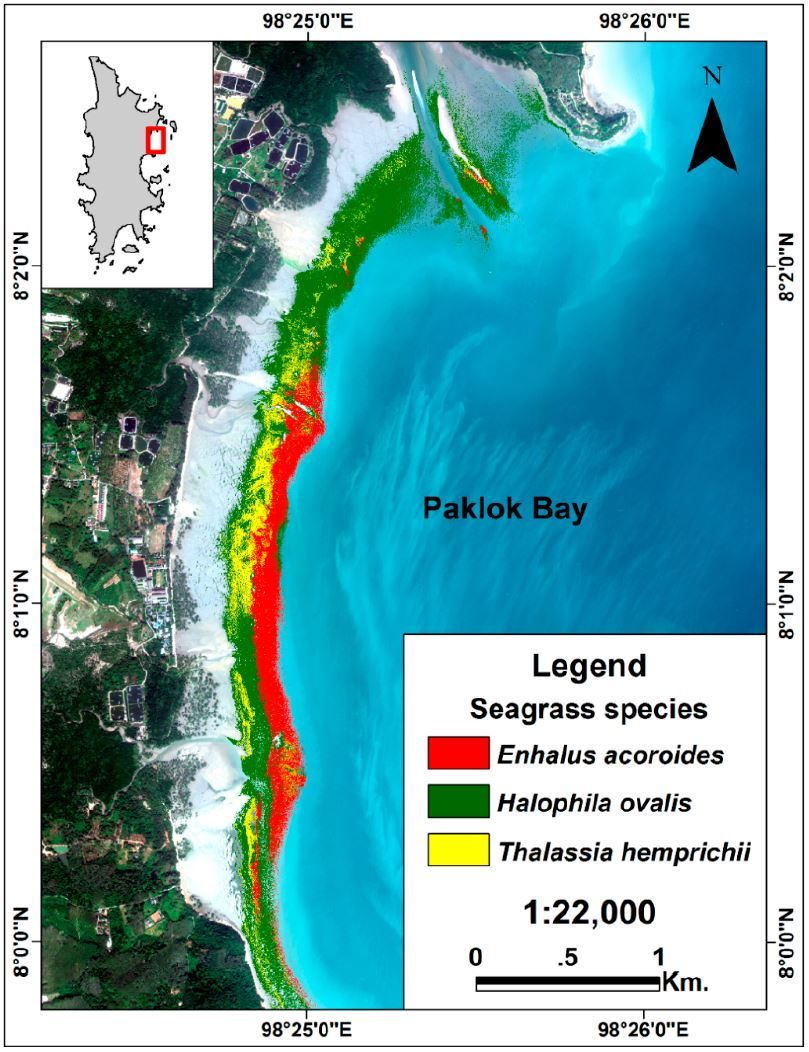
\includegraphics[width=0.7\linewidth,keepaspectratio]{./1_intro/remote_sensing_Koedsin2016}
		\caption[Exemple de cartographie d’herbiers sous-marins par télédétection]{Exemple de cartographie d’herbiers sous-marins dérivée d’images Worldview-2 et de données de référence \textit{in situ} en Thaïlande \citep{koedsin_integrated_2016}.}
	\label{figure_intro8}
\end{center}
\end{figure}

De façon similaire à la télédétection satellitaire, l’acquisition de données aériennes s’est largement développée en écologie grâce à la démocratisation des drones \citep{ivosevic_use_2015}, qui permettent d’acquérir à moindre coût des images aériennes à très haute résolution. Ce type d’image est notamment utilisé en milieu corallien pour cartographier les récifs \citep{casella_mapping_2017, collin_very_2018}.

\paragraph{Imageries sondeur et sonar : une échographie des fonds marins}

Bien que l’eau soit translucide, elle absorbe une grande proportion des rayons lumineux qui la traversent \citep{wozniak_light_2007}. Cette propriété limite considérablement les applications de la télédétection satellitaire et aérienne, qui n’est plus applicable dès lors que la profondeur ou la turbidité devient trop importante. Dans ce cas, la télédétection acoustique active (émission d’un signal de fréquence et d’intensité connues, et mesure de la réponse) à l’aide d’un capteur immergé représente une alternative à la télédétection satellite ou aérienne. Le sonar latéral et le sondeur multifaisceaux sont tous les deux des méthodes de télédétection acoustique active couramment utilisées pour cartographier les fonds marins \citep{saxena_review_1999, brown_benthic_2011} (\autoref{figure_intro9}). 

%%%%%%%%%%%%%%%%%%%%%%%%%%%%%%%%%%%%
%%% Figure intro9: Sonar sondeur %%%
%%%%%%%%%%%%%%%%%%%%%%%%%%%%%%%%%%%%
\begin{figure}[H]
	\begin{center}
	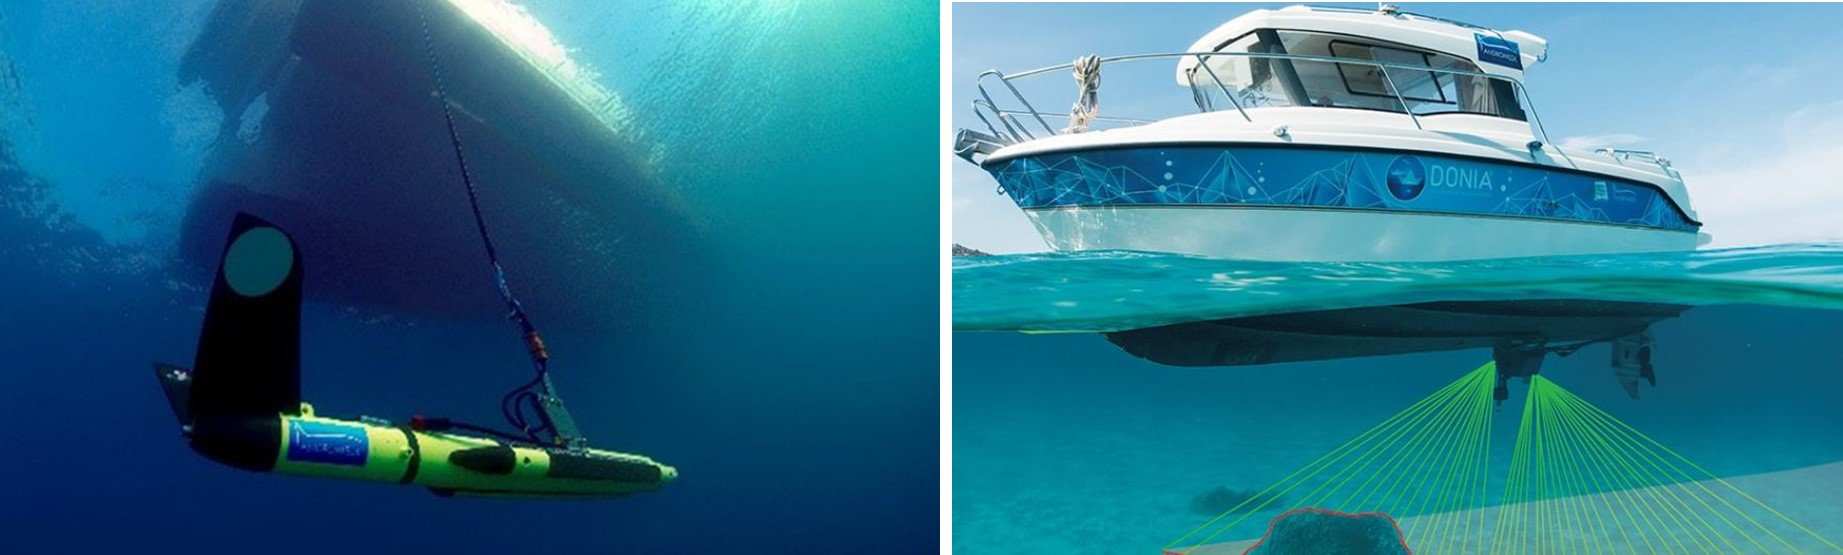
\includegraphics[width=\linewidth,keepaspectratio]{./1_intro/sonar_sondeur}
		\caption[Imagerie par sonar latéral et sondeur multifaisceaux]{Imagerie par sonar latéral (gauche) et sondeur multifaisceaux (droite) (\textit{©Andromède Océanologie}).}
	\label{figure_intro9}
\end{center}
\end{figure}

Si les deux techniques utilisent toutes deux l’acoustique, elles ne fonctionnent pas de la même manière et fournissent des résultats de natures différentes :

\begin{itemize}
    \item \textbf{Sonar latéral} : il émet un cône d’impulsions sonores d’environ 100 – 500 kHz en direction du fond et analyse l’intensité des réflexions avec une série d’hydrophones \citep{brown_benthic_2011}. Il en ressort une cartographie de l’état de surface et de la nature du fond, avec un signal d’autant plus fort que la surface du fond est dense et lisse (\autoref{figure_intro10} gauche);
    
    \item \textbf{Sondeur multifaisceaux} : il émet un cône d’impulsions sonores comme le sonar latéral, mais celui-ci mesure le temps mis par chaque impulsion pour traverser la colonne d’eau, se réfléchir sur le fond et revenir, et en déduit la profondeur en chaque point d’impact \citep{brown_benthic_2011}. Il en ressort une cartographie bathymétrique (\autoref{figure_intro10} droite).
    
\end{itemize}


%%%%%%%%%%%%%%%%%%%%%%%%%%%%%%%%%%%%%%%%%%%%%%%%%%
%%% Figure intro10: Acquisitions sonar sondeur %%%
%%%%%%%%%%%%%%%%%%%%%%%%%%%%%%%%%%%%%%%%%%%%%%%%%%
\begin{figure}[H]
	\begin{center}
	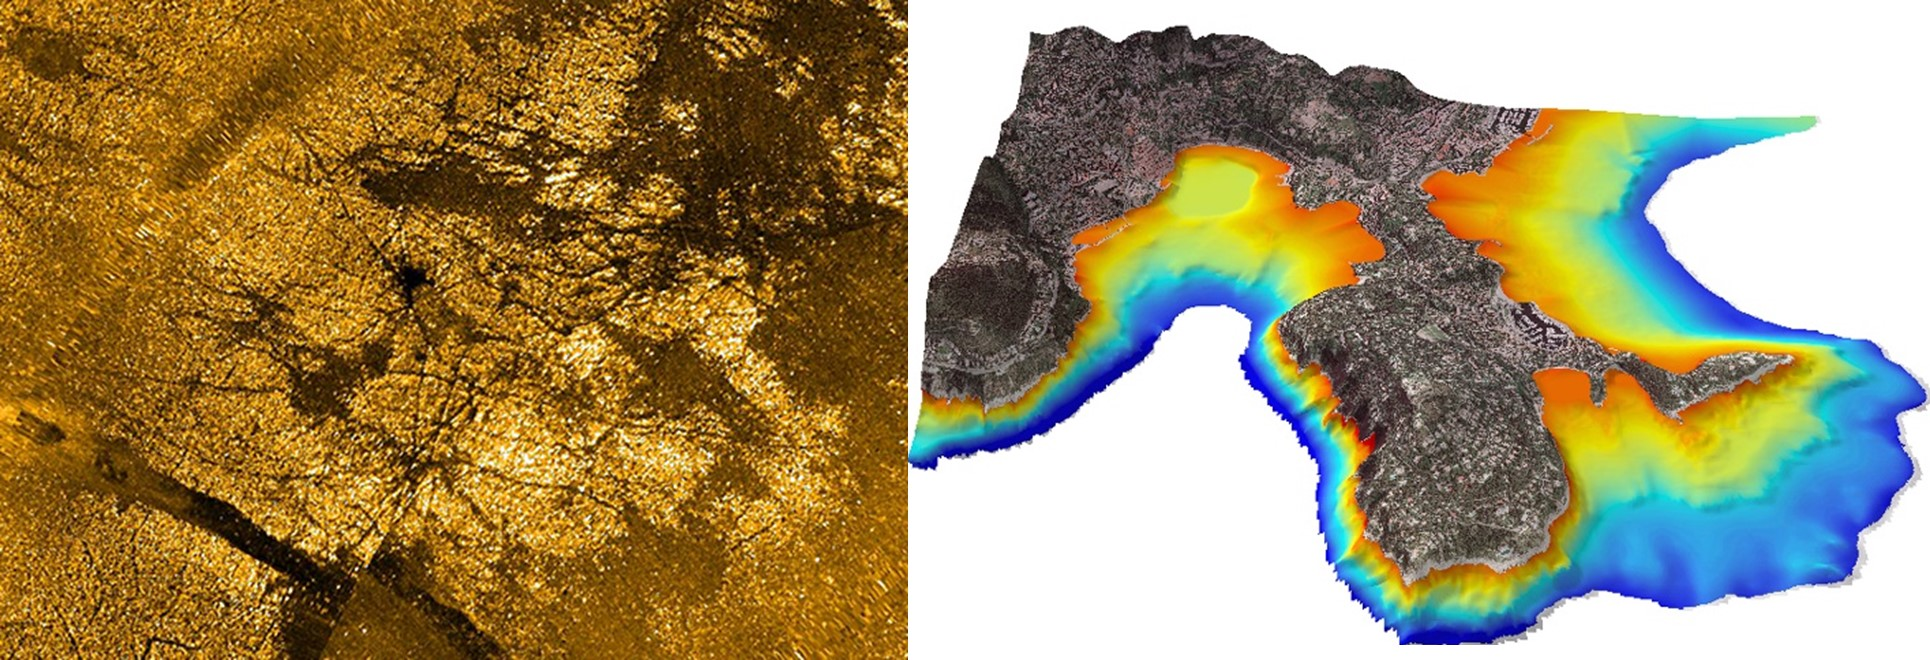
\includegraphics[width=\linewidth,keepaspectratio]{./1_intro/acquisitions_acoustiques}
		\caption[Exemples d’acquisitions acoustiques par sonar latéral et sondeur multifaisceaux]{Exemples d’acquisitions acoustiques par sonar latéral et sondeur multifaisceaux. À gauche : traces de mouillage dans l’herbier de posidonie visibles au sonar ; à droite : reproduction de la bathymétrie de Saint-Jean-Cap-Ferrat au sondeur multifaisceaux, le bleu correspondant aux zones les plus profondes (\textit{©Andromède Océanologie}).}
	\label{figure_intro10}
\end{center}
\end{figure}

Ces deux techniques sont complémentaires, elles permettent de définir des zones géographiques homogènes, identifiables par l’analyse de l’image sonar et par des observations \textit{in situ} collectées ponctuellement sur la zone d’étude \citep{brown_benthic_2011}. 

\paragraph{Caméra tractée}

De la même manière qu’un sonar est tracté derrière un bateau de sorte qu’il navigue à une dizaine de mètres au-dessus du fond, il est possible de tracter une caméra fixée sur un dispositif lui permettant de naviguer entre deux eaux et rester à distance réduite du fond \citep{rende_advances_2015}. Ce type d’acquisition photo ou vidéo permet de réaliser des assemblages photos ou des reconstructions trois dimensions (3D) des fonds par photogrammétrie et de cartographier les habitats de profondeur intermédiaire (10 – 40 m de profondeur). Comme pour le sonar latéral, il est possible d’estimer précisément la position géographique de la caméra à partir d’un positionnement GPS du bateau, du cap, de la longueur du câble et de la profondeur du dispositif (\autoref{figure_intro11}).

%%%%%%%%%%%%%%%%%%%%%%%%%%%%%%%%%%%%%%
%%% Figure intro11: Caméra tractée %%%
%%%%%%%%%%%%%%%%%%%%%%%%%%%%%%%%%%%%%%
\begin{figure}[H]
	\begin{center}
	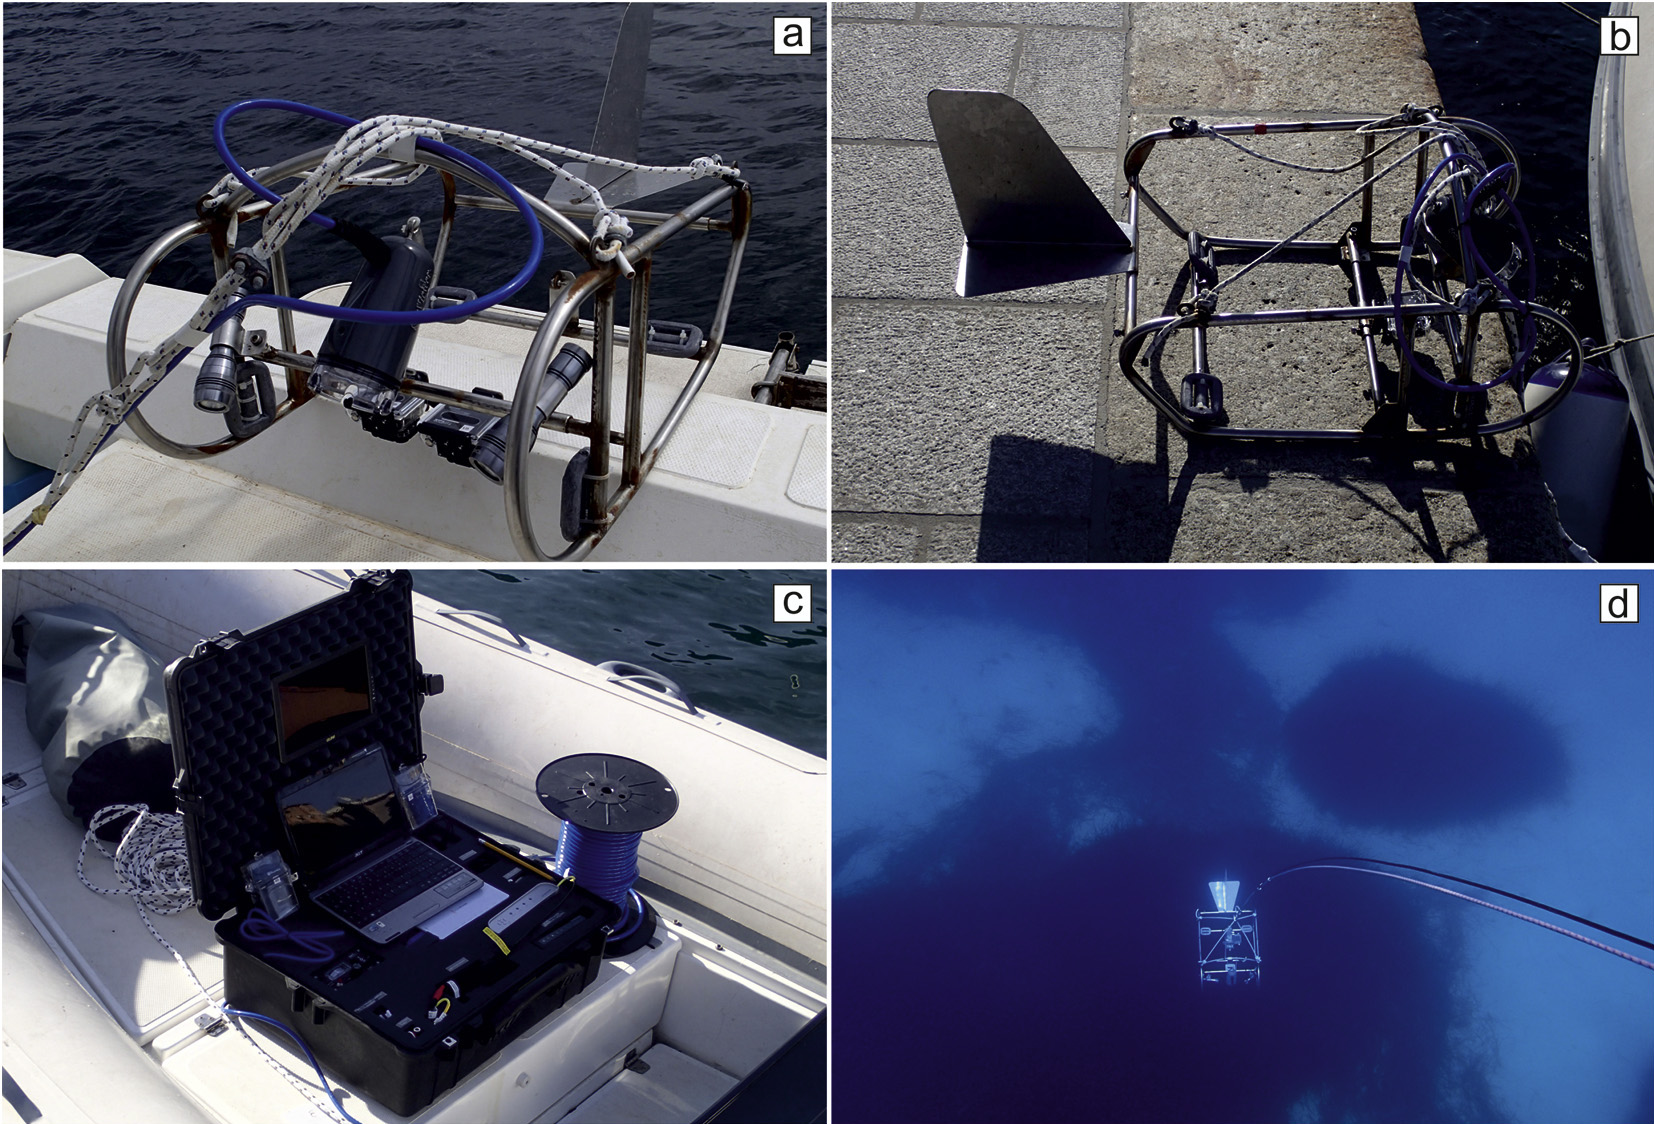
\includegraphics[width=0.7\linewidth,keepaspectratio]{./1_intro/towed_camera_Rende2015}
		\caption[Prototype de caméra tractée pour la cartographie d’habitats de profondeur intermédiaire]{Prototype de caméra tractée pour la cartographie d’habitats de profondeur intermédiaire \citep{rende_advances_2015}.}
	\label{figure_intro11}
\end{center}
\end{figure}

\setlength{\fboxsep}{5pt}
\setlength{\fboxrule}{0.6pt}
\noindent\framebox{%
  \begin{minipage}{\linewidth}
    Si les données obtenues par télédétection, quelle que soit leur nature, permettent de réaliser des cartographies à \textbf{méso/macro-échelle} pour un \textbf{coût et un temps d’acquisition relativement faibles}, elles ne permettent pas d’étudier les phénomènes écologiques qui se produisent à \textbf{micro-échelle} ni de suivre la \textbf{composition des assemblages} dans le temps.
  \end{minipage}
}

\subsubsection{Cartographie micro-échelle par proxy-détection et mesures in situ}\label{intro.2.2.2}

Si la télédétection permet d’étudier la répartition des espèces et des habitats dans l’espace, certaines études nécessitent de collecter de la donnée cartographique à plus fine échelle, comme la reconnaissance d’espèces et des mesures de tailles. Pour ces études, il est possible de réaliser des mesures \textit{in situ} ou à proximité (proxy-détection) en rapprochant le capteur du sujet.

\paragraph{Relevés plongeur}

À l’instar des relevés terrain terrestres (botanique, géologie…), l’acquisition de données peut être réalisée par le biologiste en milieu sous-marin à l’aide d’outils de plongée. Si la plongée en apnée ou sous cloche existe depuis l’Antiquité, il faudra attendre la fin du 18e siècle pour voir arriver les premiers scaphandres permettant de plus longues immersions. Plus récemment, la plongée militaire et la plongée technique ont contribué à mettre au point des scaphandres recycleurs autonomes permettant de rester plusieurs heures sous l’eau et d’atteindre des profondeurs pouvant dépasser les 100 m de fond \citep{sieber_review_2010}. Parmi la multitude de protocoles possibles, la plongée permet notamment de réaliser des relevés photographiques et de cartographier les habitats par télémétrie acoustique.

\noindent\textbf{Relevés photographiques}

Les relevés photographiques \textit{in situ} permettent de rendre compte de l’état d’un habitat à un instant donné, et de produire une évaluation qualitative (rendu visuel) ou quantitative (analyse ou interprétation d’images). Ils permettent de réaliser des assemblages photos 2D ou des reconstructions 3D (par photogrammétrie) afin de cartographier les habitats, quantifier le fractionnement, positionner les différentes espèces dans l’espace, et assurer un suivi dans le temps. Par ailleurs, la standardisation des conditions d’acquisition (distance, éclairement) permet de définir des protocoles d’échantillonnage par quadrats photographiques pour évaluer et suivre la biodiversité des habitats benthiques \citep{deter_rapid_2012} (\autoref{figure_intro12}).

%%%%%%%%%%%%%%%%%%%%%%%%%%%%%%%%%%%%%%%%%%%%%%
%%% Figure intro12: Quadrat photographique %%%
%%%%%%%%%%%%%%%%%%%%%%%%%%%%%%%%%%%%%%%%%%%%%%
\begin{figure}[H]
	\begin{center}
	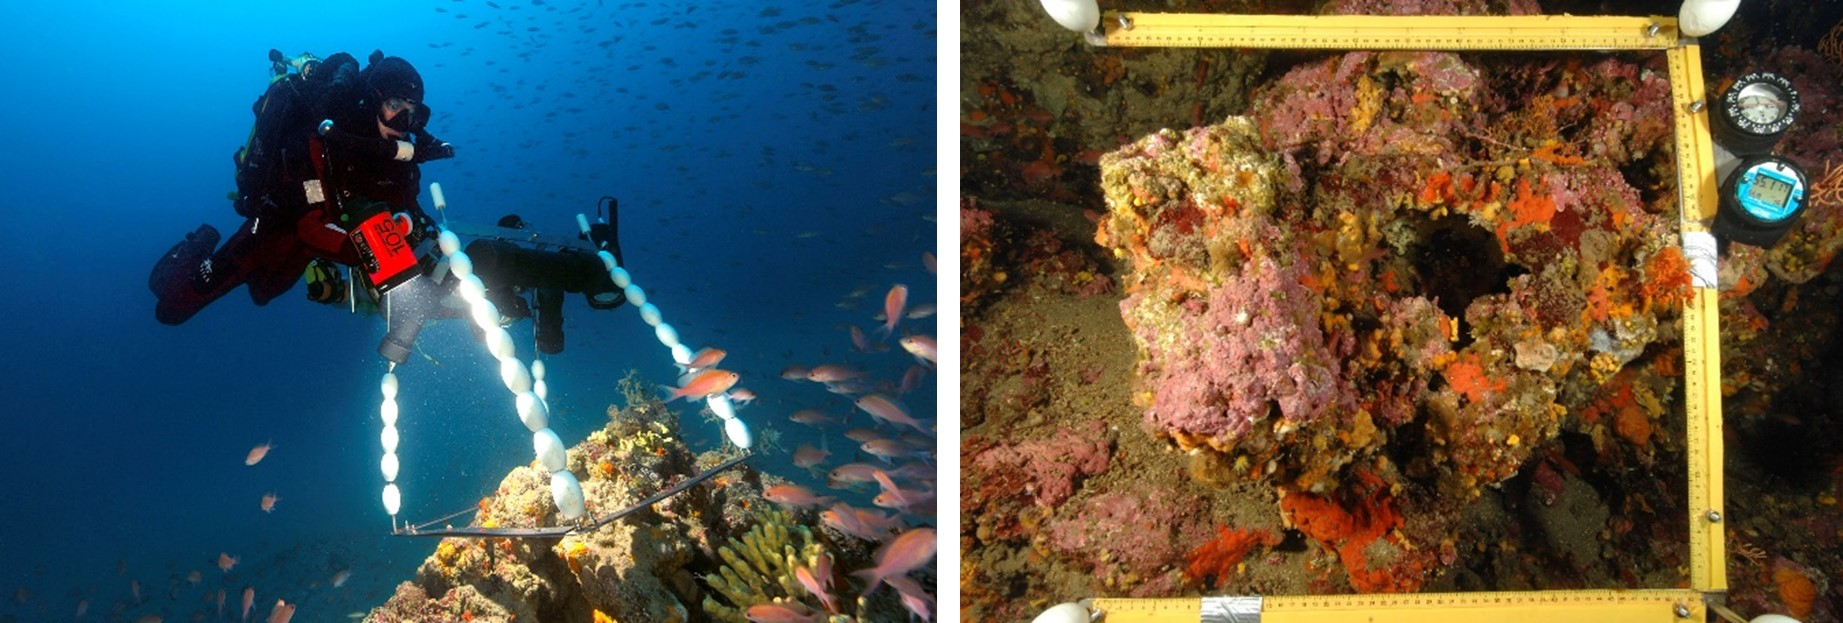
\includegraphics[width=\linewidth,keepaspectratio]{./1_intro/quadrat}
		\caption[Quadrat photographique permettant l’analyse de la biodiversité benthique par un taxonomiste]{Quadrat photographique permettant l’analyse de la biodiversité benthique par un taxonomiste (\textit{©Andromède Océanologie}).}
	\label{figure_intro12}
\end{center}
\end{figure}

\noindent\textbf{Cartographie par télémétrie acoustique}

Le signal GPS n’étant pas disponible sous l’eau, le positionnement est nécessairement relatif à une position connue (par cartographie sondeur préalable, position en surface ou bien référentiel arbitraire) et déterminé par interférométrie acoustique Ultra-Short Base Line (USBL). Ce type de technologie permet de mesurer un cap et une distance entre un émetteur et un récepteur, et donc de connaître la position d’un objet relativement à un point fixe. À l’aide de cette technologie, il est possible de cartographier des habitats marins sur une surface réduite (quelques dizaines à quelques centaines de m²) en disposant une antenne de réception fixe et en pointant la limite des objets avec un émetteur (\autoref{figure_intro13}). Les cartographies produites à différents pas de temps peuvent ensuite être géoréférencées à l’aide de points de position géographique connue (roches, aménagements…) ou bien simplement alignées et comparées, par exemple dans le cas de suivis temporels d’herbiers de posidonie \citep{descamp_underwater_2005, descamp_fast_2011}.

%%%%%%%%%%%%%%%%%%%%%%%%%%%%%%%%%%%%%%%%%%%%%
%%% Figure intro13: Télémétrie acoustique %%%
%%%%%%%%%%%%%%%%%%%%%%%%%%%%%%%%%%%%%%%%%%%%%
\begin{figure}[H]
	\begin{center}
	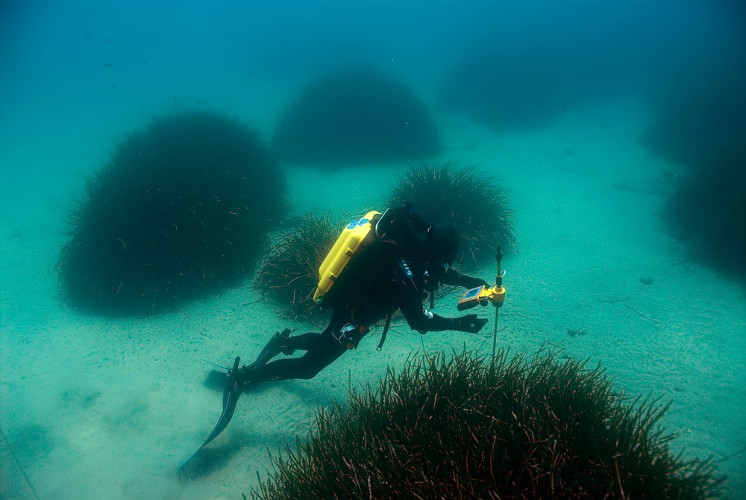
\includegraphics[width=0.8\linewidth,keepaspectratio]{./1_intro/telemetrie}
		\caption[Plongeur entrain de cartographier un herbier de posidonie à l’aide d’un télémètre acoustique]{Plongeur entrain de cartographier un herbier de posidonie à l’aide d’un télémètre acoustique (\textit{©Andromède Océanologie}).}
	\label{figure_intro13}
\end{center}
\end{figure}

\setlength{\fboxsep}{5pt}
\setlength{\fboxrule}{0.6pt}
\noindent\framebox{%
  \begin{minipage}{\linewidth}
    Si la plongée scientifique permet au naturaliste de faire lui-même ses observations et d’acquérir de la \textbf{donnée très fine}, elle est malheureusement contrainte par la \textbf{physiologique humaine} et les temps de décompression, qui augmentent exponentiellement avec la profondeur et peuvent pénaliser un plongeur durant \textbf{plusieurs heures} pour \textbf{quelques dizaines de minutes de travail} au fond. C’est pourquoi dans les cas extrêmes ou lorsque la complexité de la tâche le permet, les robots sont préférés aux plongeurs.
  \end{minipage}
}

\paragraph{Les robots: ROV et AUV}

Les robots sous-marins sont des plateformes mobiles au service de l’utilisateur, souvent adaptables pour la tâche souhaitée en les équipant du capteur ou de l’outil adéquat pour mener à bien sa mission. Si le coup de mise en œuvre est généralement élevé par rapport à un plongeur (coût du robot et déploiement par un navire océanographique adéquat), ils peuvent travailler plus profond (jusqu’à plusieurs centaines de mètres) et sans limites de temps due à la physiologie. Il en existe deux sortes : les Remotely Operated Vehicles (ROVs) et les Autonomous Underwater Vehicles (AUVs) \citep{bogue_underwater_2015}. Les ROVs sont téléopérés depuis la surface par un câble, appelé communément « ombilical », de diamètre variable selon qu’il véhicule uniquement les ordres de navigation ou bien également l’alimentation électrique. Si l’ombilical qui les relie au navire leur confère un certain handicap, il est possible de les piloter en temps réel et d’adapter la navigation et l’acquisition de données en fonction de ce que voit le pilote en surface (\autoref{figure_intro14}).

%%%%%%%%%%%%%%%%%%%%%%%%%%%%%
%%% Figure intro14: ROV3D %%%
%%%%%%%%%%%%%%%%%%%%%%%%%%%%%
\begin{figure}[H]
	\begin{center}
	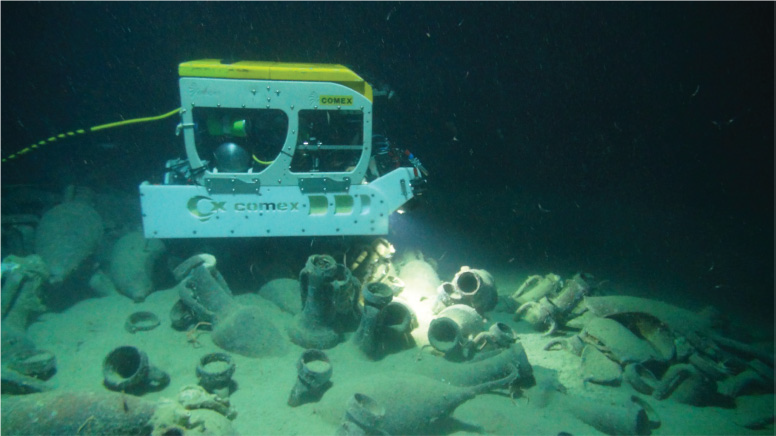
\includegraphics[width=0.7\linewidth,keepaspectratio]{./1_intro/ROV3D_Drap2015}
		\caption[ROV3D : un robot d’acquisition photogrammétrique pour l’archéologie sous-marine]{ROV3D : un robot d’acquisition photogrammétrique pour l’archéologie sous-marine \citep{drap_rov_2015}.}
	\label{figure_intro14}
\end{center}
\end{figure}

Comme leur nom l’indique, les AUVs sont autonomes et doivent donc être programmés pour réaliser un parcours d’acquisition précis et maintenir une distance au fond tout en évitant les éventuels obstacles, en utilisant des technologies de positionnement \citep{johnson-roberson_generation_2010, bonin-font_towards_2016} (\autoref{figure_intro15}). Ces robots permettent de réaliser des acquisitions de manière entièrement autonome une fois déployés, mais ils requièrent une technologie et un temps de développement généralement beaucoup plus onéreux que les ROVs.

%%%%%%%%%%%%%%%%%%%%%%%%%%%
%%% Figure intro15: AUV %%%
%%%%%%%%%%%%%%%%%%%%%%%%%%%
\begin{figure}[H]
	\begin{center}
	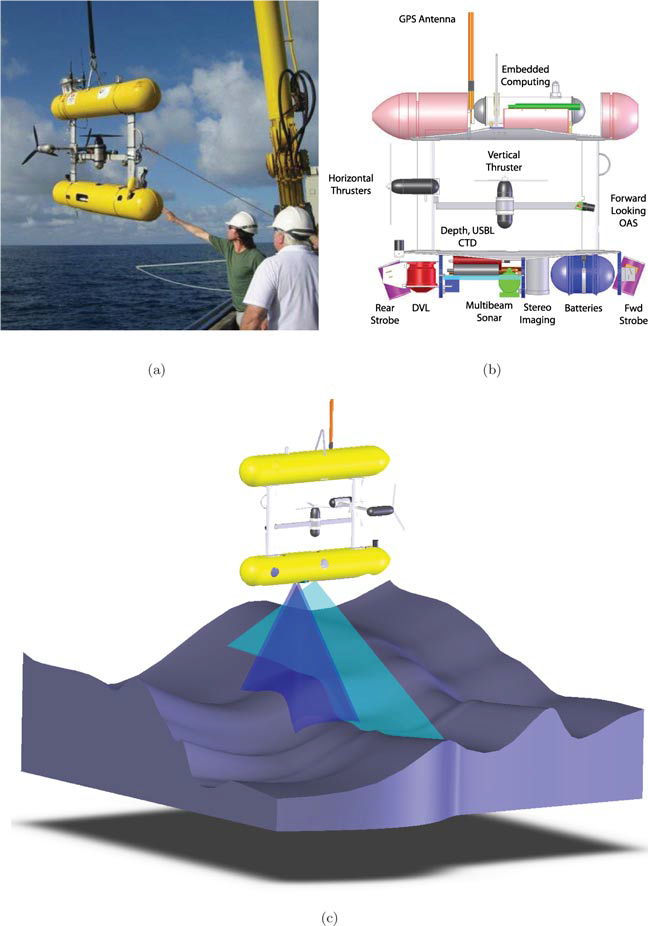
\includegraphics[width=0.7\linewidth,keepaspectratio]{./1_intro/AUV_Johnson-Roberson2010}
		\caption[Exemple d’un robot autonome (AUV) pour de l’acquisition d’images à grande échelle]{Exemple d’un robot autonome (AUV) pour de l’acquisition d’images à grande échelle \citep{johnson-roberson_generation_2010}.}
	\label{figure_intro15}
\end{center}
\end{figure}

\setlength{\fboxsep}{5pt}
\setlength{\fboxrule}{0.6pt}
\noindent\framebox{%
  \begin{minipage}{\linewidth}
    Les robots sous-marins sont d’excellents outils pour acquérir des données photographiques sur de \textbf{grandes surfaces} (AUV) ou à de \textbf{grandes profondeurs} (ROV) ; mais leur maniabilité réduite, leur coût de développement et leur mise en œuvre rendent bien souvent le \textbf{plongeur autonome plus pertinent} et compétitif (jusqu’à une certaine profondeur), notamment depuis la démocratisation des scaphandres recycleurs. 
  \end{minipage}
}

\subsection{Les réseaux de surveillance en Méditerranée française}\label{intro.2.3}

Les réseaux de surveillance ont pour objectif le suivi écologique de certains habitats ou espèces à l’échelle régionale ou globale, en standardisant les méthodes de collecte et de traitement de données. L’analyse des données de ces réseaux permet de comparer la qualité écologique des différentes stations de suivis et de mesurer leur évolution dans le temps, afin de mettre en œuvre des mesures de gestion efficaces. De nombreux réseaux de surveillance existent en Méditerranée française, dont une partie est financée par l’Agence de l’Eau Rhône-Méditerranée-Corse, et sont rassemblés sur la plateforme cartographique « Medtrix » (\href{https://medtrix.fr/}{https://medtrix.fr/}). Deux de ces réseaux sont gérés par la société Andromède Océanologie et concernent les habitats les plus riches et les plus sensibles de Méditerranée : les herbiers de posidonie (TEMPO) et les récifs coralligènes (RECOR).

\subsubsection{La société Andromède Océanologie}\label{intro.2.3.1}

Andromède Océanologie (\href{www.andromede-ocean.com}{www.andromede-ocean.com}) est une PME créée en 2008, spécialisée dans les relevés écologiques \textit{in situ} en plongée sous-marine. Son objectif est de conduire des projets innovants liés à l'étude et à la valorisation de l'environnement marin. Les activités d’Andromède Océanologie et de son équipe de 13 personnes sont organisées en 3 pôles : 

\begin{itemize}
    \item \textbf{Un pôle bureau d’études} dont les capacités d’expertise ont notamment trait à la bathymétrie, la cartographie des biocénoses marines, l’analyse écologique et la gestion des écosystèmes marins~;
    
    \item \textbf{Un pôle valorisation} qui gère notamment la diapothèque (plus de 25 000 clichés) de Laurent Ballesta, plongeur extrême et photographe sous-marin internationalement reconnu, auteur de nombreux livres, documentaires et expéditions~;
    
    \item \textbf{Un pôle Recherche et Développement} qui met au point des technologies innovantes pour l’évaluation, le suivi et l’amélioration de l’état de santé des écosystèmes marins côtiers. Andromède porte ainsi plusieurs réseaux de surveillance de l’état écologique des eaux côtières, en partenariat avec l’Agence de l’Eau Rhône Méditerranée Corse. Par ailleurs, un programme de « laboratoire commun » mutualise les moyens et efforts de recherche entre la société et l’Université de Montpellier (UMR MARBEC) pour le développement de méthodes d’observations innovantes sur les habitats méditerranéens\\ (\href{https://labcomintosea.edu.umontpellier.fr}{https://labcomintosea.edu.umontpellier.fr}).
\end{itemize}

La société est localisée en bord de mer à Carnon (Occitanie, France), et dispose d’un parc matériel et technologique très spécialisé consacré aux domaines de l'océanologie et de la plongée hi Tech : trois bateaux, sonar latéral, sondeur multifaisceaux, système de positionnement GPS-rtk, scaphandres de plongée à circuit ouvert et fermé (recycleur), équipement photo et vidéo sous-marines pour films professionnels, etc. Andromède Océanologie a réalisé la plupart des cartographies des biocénoses marines côtières (0 à 80 m de fond) de Méditerranée française et quelques zones à l’étranger (ilots de Galite et Zembra en Tunisie, réserves de Tavolara et Carbonara en Sardaigne (Italie), réserve de Karaburun - Sazan en Albanie, etc.). Elle est à l’origine de la première cartographie continue des biocénoses (1 : 10 000) en Méditerranée française (Andromède Océanologie, 2014). Ces cartes sont mises gratuitement à la disposition des professionnels de la mer sur la plateforme cartographique Medtrix (\href{https://plateforme.medtrix.fr/}{https://plateforme.medtrix.fr/}) dans le projet DONIA Expert. Une version simplifiée de ces cartes est disponible sur l’application mobile de plaisance Donia : ancrage en toute sécurité et hors des habitats sensibles, cartes 3D des fonds pour repérer les sites de plongée ou de pêche, outil de navigation communautaire… (\href{https://donia.fr/}{https://donia.fr/}) Cette application gratuite a reçu le prix Bateau Bleu et le prix Entreprises et Biodiversité de 2013, et a fait l’objet d’une mise à jour (version 5.0) importante en 2020 (ajout de données et d’outils, amélioration de l’ergonomie).

\subsubsection{TEMPO : un réseau de surveillance des herbiers de posidonie en Méditerranée française}\label{intro.2.3.2}

Les herbiers sous-marins sont de bons indicateurs des conditions environnementales : une perturbation de leur distribution traduit des changements environnementaux \citep{orth_global_2006}. Plus particulièrement, la posidonie, qui pousse à des profondeurs allant de la surface jusqu’à plus de 40 m de fond en fonction de la clarté de l’eau, est couramment utilisée comme un bio-indicateur de la qualité de l’eau, entre autres à travers l’évolution de sa limite inférieure (i.e. limite profonde au-delà de laquelle les conditions favorables à sa croissance ne sont plus réunies) \citep{boudouresque_regression_2009, ruiz_mediterranean_2009}. En effet, la profondeur de la limite inférieure est principalement déterminée par la clarté de l’eau, et représente un indicateur robuste de l’état global de l’ensemble de l’écosystème \citep{borum_european_2004}. Par ailleurs, il est important de prendre en compte des mesures quantitatives de la vitalité de l’herbier à une profondeur identique (-15 m ; profondeur représentative de l’herbier en Méditerranée), car les herbiers peu profonds montrent une grande variabilité naturelle \citep{marba_interannual_1997, balestri_spatial_2003}. Des indicateurs intègrent les différentes mesures de vitalité de l’herbier (densité, longueurs de feuilles, épiphytes…) et des espèces associées (herbivores, échinodermes, filtreurs, prédateurs…), afin d’évaluer le fonctionnement global de l’herbier, à la fois à la profondeur intermédiaire et en limite inférieure.

TEMPO est un réseau de surveillance de l’état écologique des herbiers de posidonie en Méditerranée française qui intègre ces deux composantes importantes de l’herbier : la limite inférieure et la profondeur intermédiaire. Ce réseau est opéré par Andromède océanologie, depuis 2011, avec le soutien de l’Agence de l’Eau Rhône-Méditerranée-Corse. La caractérisation de l’état écologique de l’herbier est réalisée par une campagne régionale annuelle sur la période mi-mai / fin juin. Chaque année, une des trois régions concernées par cette agence de l’eau (Corse, région Sud-Provence-Alpes Côte d’Azur et Occitanie) est échantillonnée, avec un roulement sur trois ans. Toutes régions confondues, le réseau TEMPO permet au total l’échantillonnage de 96 sites d’herbier dont 47 sites sont localisés à la profondeur intermédiaire et 53 en limite inférieure (quatre limites inférieures peu profondes sont aussi considérées comme sites à la profondeur intermédiaire), le plus souvent dans l’alignement des sites à profondeur intermédiaire (\autoref{figure_intro16}). 

%%%%%%%%%%%%%%%%%%%%%%%%%%%%%%%%%%%%%%%
%%% Figure intro16: le réseau TEMPO %%%
%%%%%%%%%%%%%%%%%%%%%%%%%%%%%%%%%%%%%%%
\begin{figure}[H]
	\begin{center}
	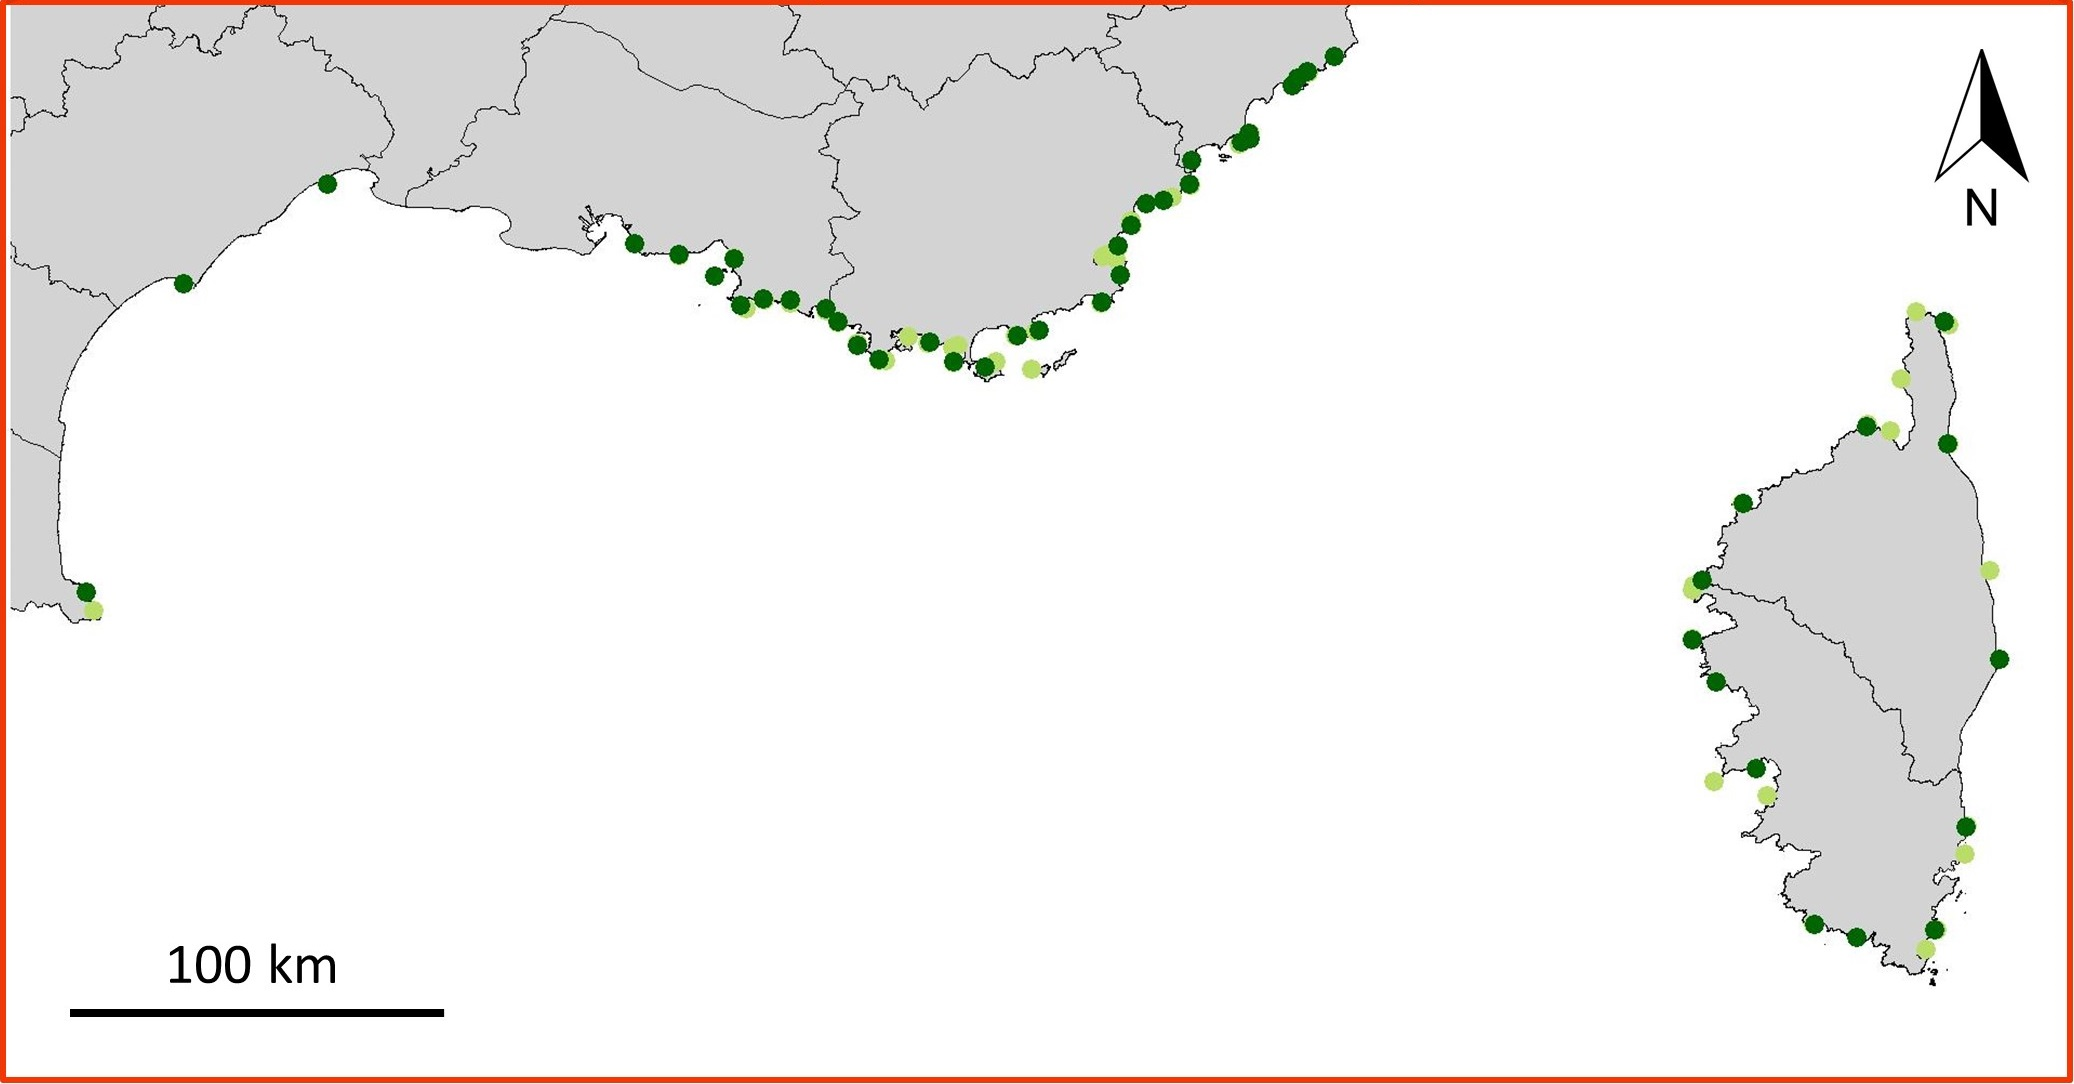
\includegraphics[width=\linewidth,keepaspectratio]{./1_intro/reseau_TEMPO}
		\caption[Localisation des sites du réseau de surveillance TEMPO]{Localisation des sites du réseau de surveillance TEMPO. En vert clair: les 47 sites à -15m ; en vert foncé: les 53 sites en limite inférieure.}
	\label{figure_intro16}
\end{center}
\end{figure}

La méthode choisie pour la surveillance de l’herbier de posidonie en limite inférieure prend en compte deux types de mesures : une cartographie de la limite inférieure de l’herbier par télémétrie acoustique, et des mesures de vitalité de l’herbier. La méthode de télémétrie acoustique permet à l’opérateur d’effectuer un point tous les 30 à 50 cm pour cartographier précisément la limite inférieure grâce à l’Aquamètre D100-NG dernière génération (\href{http://www.plsm.eu}{http://www.plsm.eu}) relié à une tablette tactile étanche. La caractérisation de l’état de conservation des herbiers de Posidonia oceanica est réalisée selon les protocoles standardisés du PREI \citep{gobert_assessment_2009}, de l’EBQI \citep{personnic_ecosystem-based_2014} et du BiPo \citep{lopez_y_royo_biotic_2010} basés sur des mesures biologiques in situ et en laboratoire. Par ailleurs, des mesures bioacoustiques sont réalisées sur certains sites afin de quantifier l’activité des espèces mobiles (en partenariat avec l’équipe de Chorus (\href{https://chorusacoustics.com/}{https://chorusacoustics.com/}) qui porte le réseau de surveillance CALME) (\autoref{figure_intro17}).

\medskip 

\setlength{\fboxsep}{5pt}
\setlength{\fboxrule}{0.6pt}
\noindent\framebox{%
  \begin{minipage}{\linewidth}
    Le protocole TEMPO permet d’acquérir une \textbf{diversité de mesures de vitalité de l’herbier} à la \textbf{profondeur intermédiaire} (-15 m) et en \textbf{limite inférieure}, ainsi que des \textbf{espèces associées} (filtreurs, herbivores…). Si la cartographie de la limite inférieure par \textbf{télémétrie acoustique} permet de suivre finement son \textbf{évolution dans le temps}, la résolution dépend de la volonté du plongeur, et la manipulation peut être longue et devenir \textbf{physiologiquement contraignante} pour le plongeur dans le cas des herbiers les plus \textbf{profonds} (notamment en Corse) et les plus \textbf{fragmentés}.
  \end{minipage}
}

%%%%%%%%%%%%%%%%%%%%%%%%%%%%%%%%%%%%%%%%
%%% Figure intro17: la méthode TEMPO %%%
%%%%%%%%%%%%%%%%%%%%%%%%%%%%%%%%%%%%%%%%
\begin{sidewaysfigure}
\begin{figure}[H]
	\begin{center}
	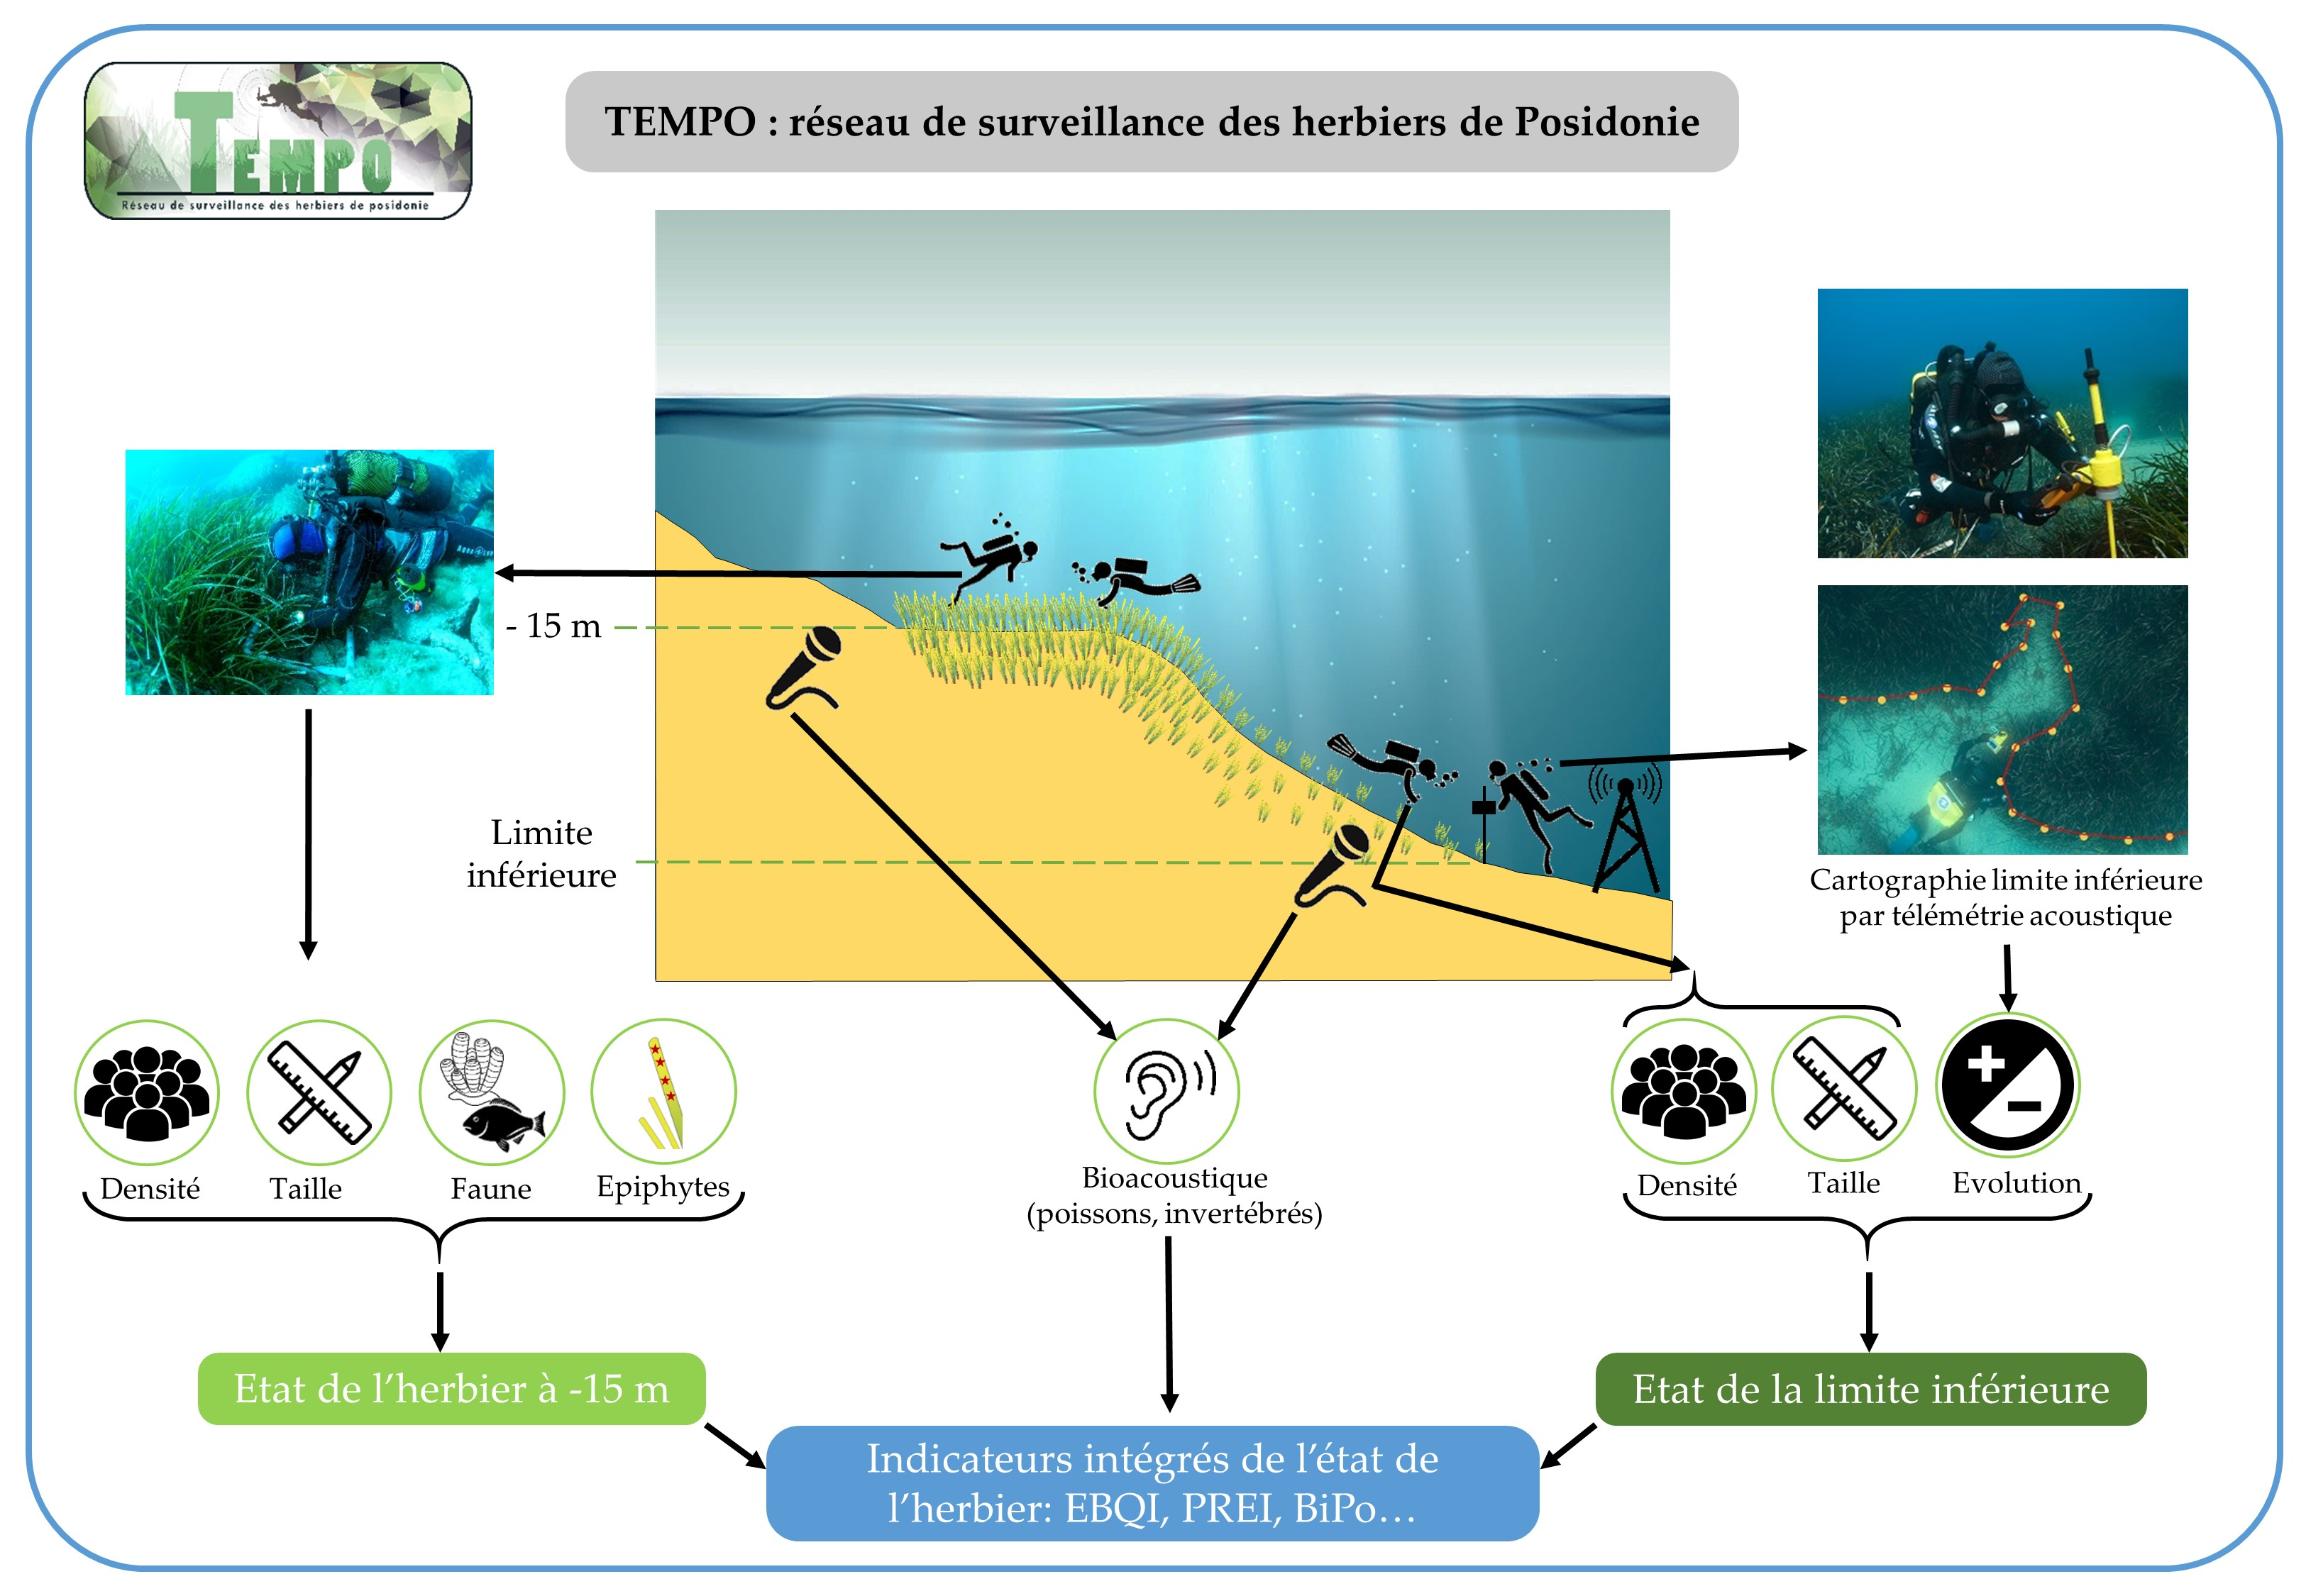
\includegraphics[width=\linewidth,keepaspectratio]{./1_intro/encart_TEMPO}
		\caption[TEMPO : réseau de surveillance des herbiers de posidonie en Méditerranée française]{TEMPO : réseau de surveillance des herbiers de posidonie en Méditerranée française.}
	\label{figure_intro17}
\end{center}
\end{figure}
\end{sidewaysfigure}

\newpage

\subsubsection{RECOR : un réseau de surveillance des assemblages des récifs coralligènes en Méditerranée française}\label{intro.2.3.3}

« Il est urgent de développer de nouvelles méthodes pour comprendre la structuration de ces assemblages [coralligènes], et évaluer les impacts auxquels ils sont soumis, afin de fournir un état de référence et explorer les possibles trajectoires d’évolution de ces assemblages d’une grande diversité » \citep{kipson_rapid_2011}. RECOR est un réseau de surveillance de l’état écologique des récifs coralligènes en Méditerranée, opéré par Andromède océanologie depuis 2010 avec le soutien de l’Agence de l’eau Rhône-Méditerranée-Corse. Comme pour TEMPO, la caractérisation de l’état écologique des récifs est réalisée par campagne régionale annuelle sur la période mi-mai / fin juin. Chaque année, une des trois régions concernées par cette agence de l’eau (Corse, région Sud-Provence-Alpes Côte d’Azur et Occitanie) est échantillonnée, avec un roulement sur trois ans. Toutes régions confondues, le réseau RECOR permet au total l’échantillonnage de 177 stations situées sur 97 sites (i.e. récifs) lors des trois années de suivi (\autoref{figure_intro18}). Les stations sont situées à des profondeurs comprises entre 17 et 90 m, et un site peut inclure plusieurs stations à des profondeurs différentes.

%%%%%%%%%%%%%%%%%%%%%%%%%%%%%%%%%%%%%%%
%%% Figure intro18: le réseau RECOR %%%
%%%%%%%%%%%%%%%%%%%%%%%%%%%%%%%%%%%%%%%
\begin{figure}[H]
	\begin{center}
	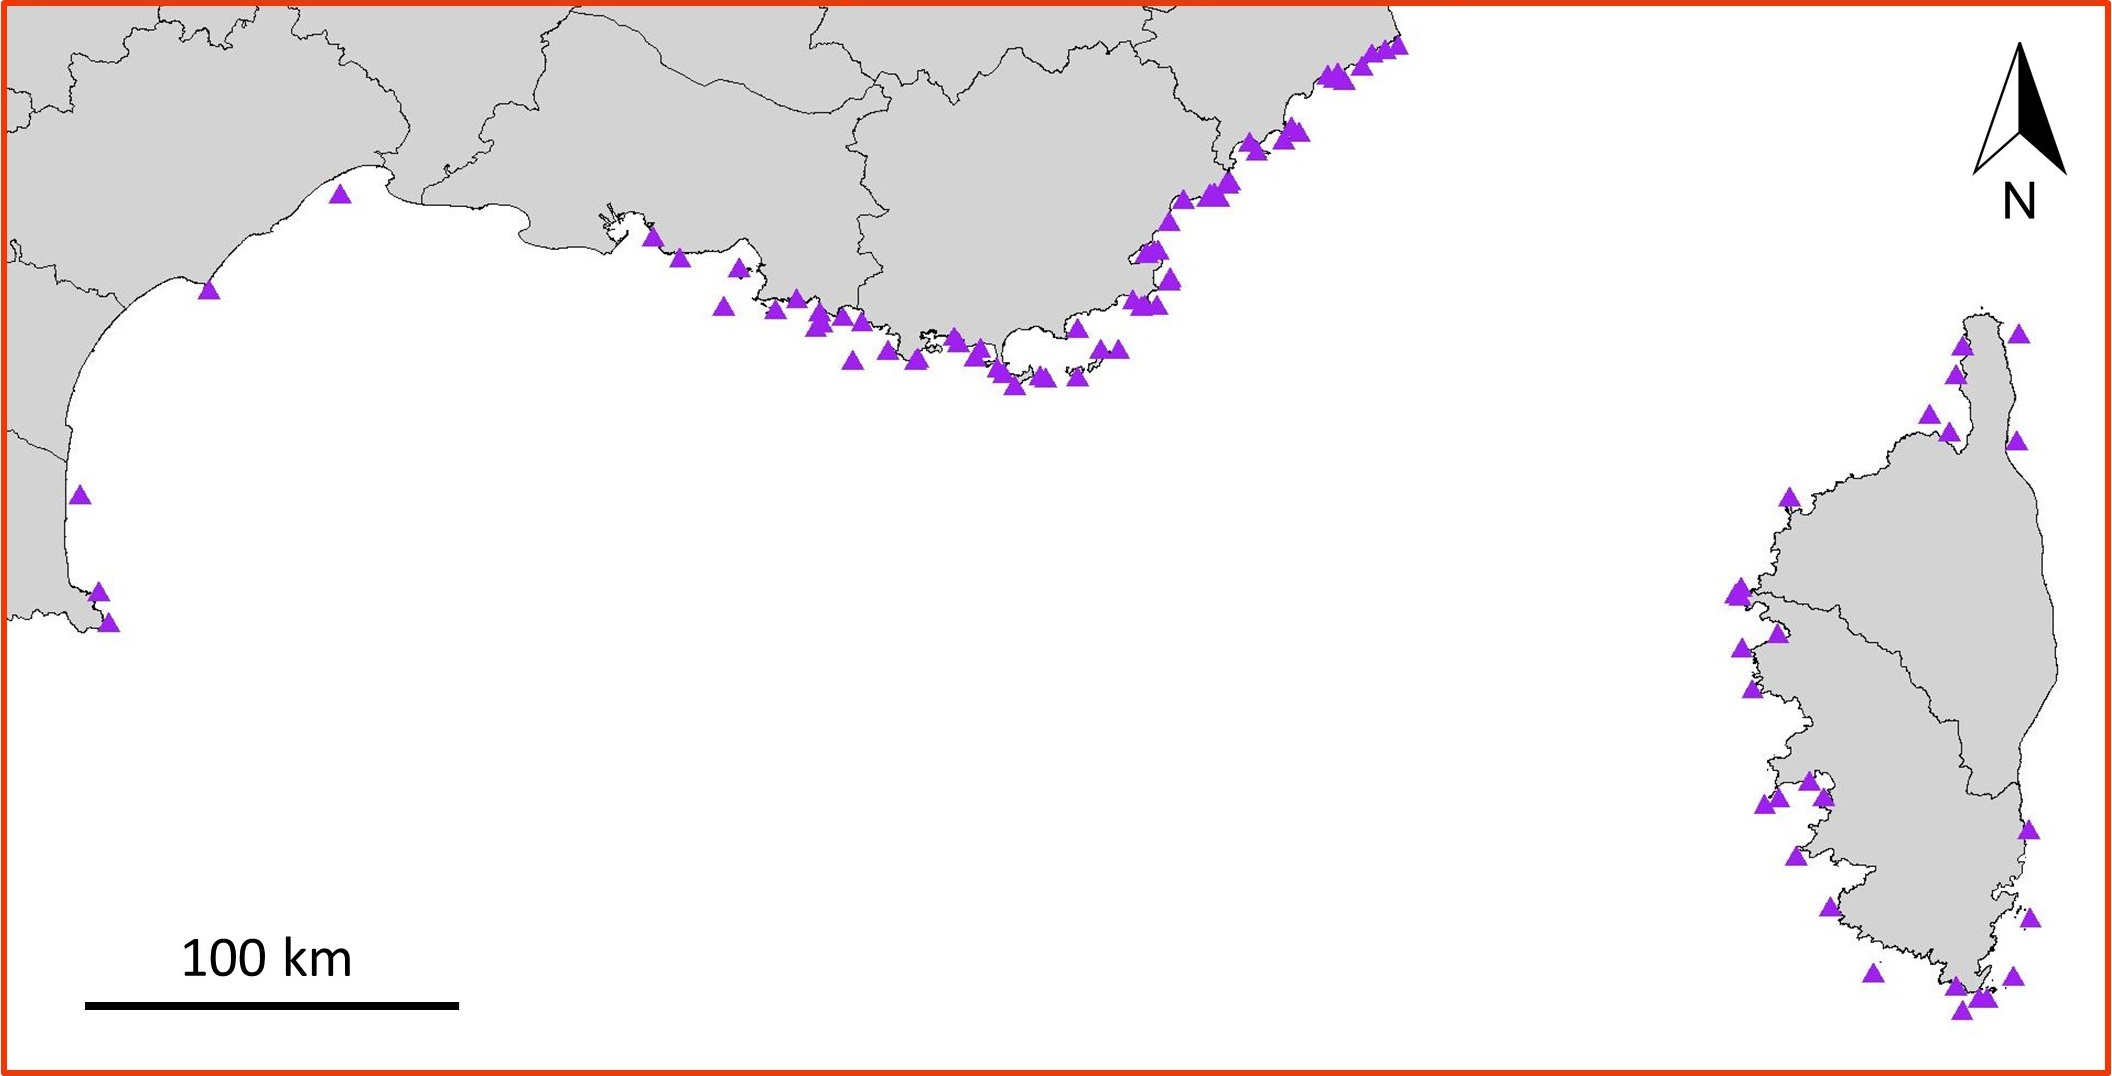
\includegraphics[width=\linewidth,keepaspectratio]{./1_intro/reseau_RECOR}
		\caption[Localisation des 97 sites du réseau de surveillance RECOR]{Localisation des 97 sites du réseau de surveillance RECOR.}
	\label{figure_intro18}
\end{center}
\end{figure}

Encore plus que pour les habitats peu profonds, le suivi des récifs coralligènes est limité par les contraintes physiologiques du plongeur. En effet, à ces profondeurs (couramment 50 à 80 m de fond), chaque minute de plongée supplémentaire nécessite un temps accru de décompression. Par conséquent, la méthode de suivi la plus utilisée est le quadrat photographique : le plongeur réalise 30 images standardisées (distance au récif et éclairage contrôlé), échantillonnées à différents endroits du récif, qui sont ensuite identifiées par un taxonomiste une fois de retour au bureau \citep{deter_rapid_2012}. Les images sont analysées à l’aide du logiciel Coral Point Count \citep{cpce_coral_2011} 4.1 « coralligenous assemblages version » en échantillonnant aléatoirement 64 points par image (soit 30 $\times$ 64 = 1920 points par station), et chaque point est identifié par le même expert taxonomiste. Celui-ci calcule ensuite, à l’échelle de la station, des indicateurs d’état de conservation et de diversité, notamment :

\begin{itemize}
    \item \textbf{Coralligenous Assemblage Index (CAI)} \citep{deter_preliminary_2012} : indicateur représentatif de l’état écologique d’un récif. Il prend en compte trois composantes : la proportion de bioconstructeurs, la proportion de vase et la proportion de bryozoaires. Chacune des trois valeurs est standardisée par la valeur minimale (pour la vase) ou maximale (pour les bioconstructeurs et les bryozoaires) mesurée par région. Il est calculé comme suit :
    
    \begin{equation}
        \text{CAI\textsubscript{i}}=\frac{1}{3}\times(\frac{1-sludge_i}{1-\min_{i}sludge_i}+\frac{majbuilders_i}{\max_{i}majbuilders_i}+\frac{bryozoans_i}{\max_{i}bryozoans_i})
        \label{eqintro.2}
    \end{equation}
    
    \item \textbf{Indice de Shannon} \citep{magurran_measuring_2004} : voir section \ref{intro.2.1}~;
    
    \item \textbf{Nécroses} : pourcentage de mortalité d’algues bioconstructrices (potentiellement lié à la température, pathogènes, pollution, compétition…)~;
    
    \item \textbf{Indice algues filamenteuses} : pourcentage d’algues filamenteuses qui prolifèrent et recouvrent les récifs (potentiellement lié à la température, nutriments et salinité).

\end{itemize}

Ces indicateurs permettent de définir un état de diversité et de conservation à un instant t, et le suivi de leur évolution dans le temps permet de quantifier la potentielle dégradation ou récupération des récifs. Conjointement à ces analyses, les plongeurs réalisent des mesures de tailles, densités et nécroses de gorgones au sein de 30 quadrats de 0,5 $\times$ 0,5 m (\autoref{figure_intro19}). Les gorgones sont des espèces érigées suspensivores sensibles aux perturbations mécaniques et aux variations de qualité de l’eau et de la température, et sont donc un bon témoin de la qualité écologique d’un récif. Enfin, comme pour le réseau TEMPO, des mesures bioacoustiques sont réalisées sur certains sites afin de quantifier l’activité des espèces mobiles (en partenariat avec l’équipe Chorus (\href{https://chorusacoustics.com/}{https://chorusacoustics.com/}) qui porte le réseau de surveillance CALME).

\medskip

\setlength{\fboxsep}{5pt}
\setlength{\fboxrule}{0.6pt}
\noindent\framebox{%
  \begin{minipage}{\linewidth}
    Le protocole RECOR permet d’acquérir en peu de temps une \textbf{grande quantité de données} indispensables à \textbf{l’évaluation de la diversité des assemblages coralligènes} et de leur \textbf{état de santé}. Cependant, l’analyse a posteriori des images pour \textbf{l’identification des espèces du coralligène} requiert des \textbf{compétences taxonomistes} et sont extrêmement \textbf{chronophage} (1 920 identifications par station sont nécessaires à l’évaluation de ces assemblages complexes).
  \end{minipage}
}

%%%%%%%%%%%%%%%%%%%%%%%%%%%%%%%%%%%%%%%%
%%% Figure intro19: la méthode RECOR %%%
%%%%%%%%%%%%%%%%%%%%%%%%%%%%%%%%%%%%%%%%
\begin{sidewaysfigure}
\begin{figure}[H]
	\begin{center}
	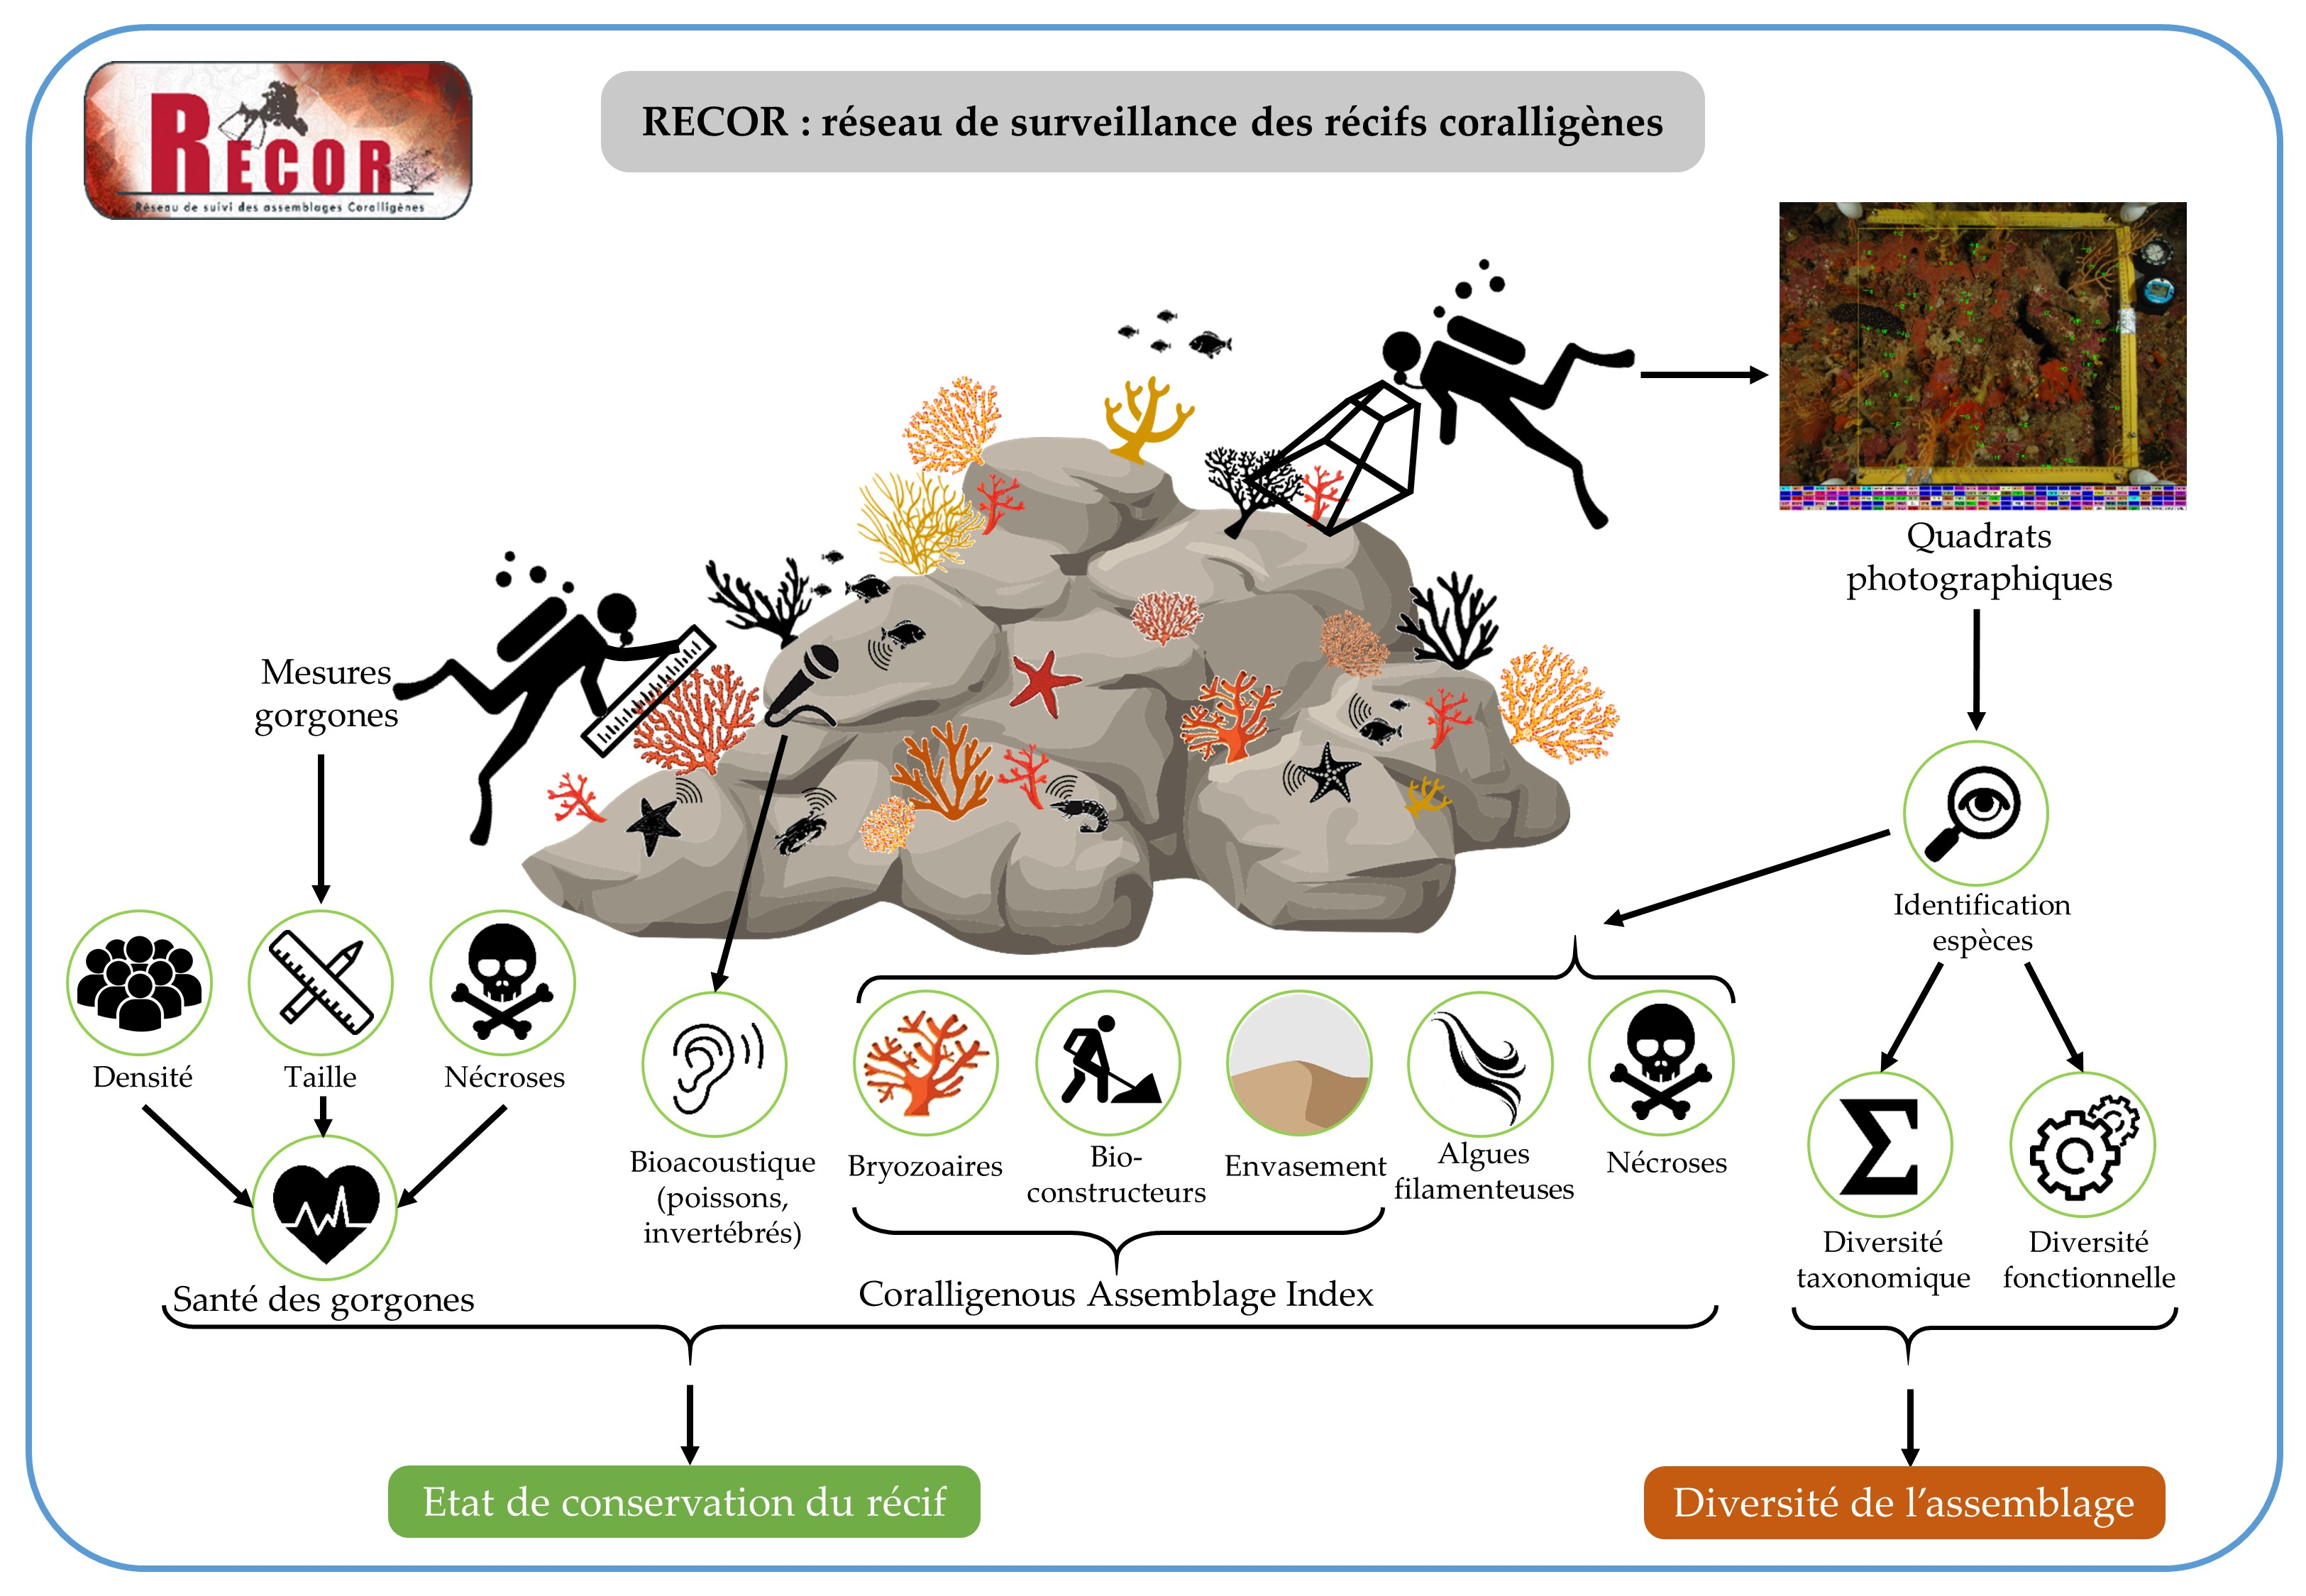
\includegraphics[width=\linewidth,keepaspectratio]{./1_intro/encart_RECOR}
		\caption[RECOR : réseau de surveillance des récifs coralligènes en Méditerranée française]{RECOR : réseau de surveillance des récifs coralligènes en Méditerranée française.}
	\label{figure_intro19}
\end{center}
\end{figure}
\end{sidewaysfigure}

\newpage

%%% PROBLEMATIQUE %%%
\section{Problématique et objectifs de la thèse}\label{intro.3}

La \textbf{biodiversité mondiale} subit actuellement d’importantes \textbf{pressions d’origine anthropique}, menant à un rythme d’extinction d’espèces et de dégradation des habitats sans précédent depuis la dernière grande extinction de masse il y a 66 millions d’années. Les \textbf{écosystèmes marins}, en particulier, qui concentrent une grande partie de la \textbf{biodiversité} et des \textbf{services écosystémiques}, souffrent du cumul de ces pressions à l’échelle globale. La mise en place de \textbf{mesures de conservation efficaces} pour limiter les impacts anthropiques sur le milieu marin est cruciale, particulièrement en \textbf{Méditerranée}, une mer qui concentre à la fois de hauts niveaux de biodiversité et d’importantes pressions cumulées. Cependant, les \textbf{difficultés d’accès} au monde sous-marin limitent considérablement l’acquisition de données et donc les connaissances sur la distribution et l’évolution de sa biodiversité. La \textbf{surveillance écologique} de ces habitats sensibles est primordiale : elle doit permettre aux décideurs et gestionnaires d’établir des \textbf{mesures de conservation} et de quantifier leur efficacité afin de limiter au maximum les impacts anthropiques sur ces habitats. C’est l’objet des deux réseaux de surveillance \textbf{TEMPO} et \textbf{RECOR}, centrés sur les \textbf{herbiers de posidonie} et les \textbf{récifs coralligènes}, les deux habitats les plus riches de Méditerranée. S’ils bénéficient d’une dizaine d’années d’expérience, ces deux réseaux sont en constante évolution. Les développements récents en matière d’analyses d’images offrent des opportunités intéressantes pour alimenter la chaîne d’\textbf{acquisition} et de \textbf{traitement} de données écologiques. Les potentialités sont une réduction des incertitudes, l’augmentation de la couverture spatiale et temporelle, et la diminution de temps de traitement par l’automatisation de traitements.

La \textbf{reconnaissance d’images} a connu une grande révolution avec le développement des premiers grands \textbf{réseaux de neurones convolutifs} au début des années 2010. Ces algorithmes, dont les performances dépassent parfois même celles d’un opérateur humain, sont de plus en plus utilisés en sciences, notamment en écologie avec la \textbf{reconnaissance d’espèces}. Dans le même temps, un autre type de traitement d’images s’est largement développé grâce à l’amélioration des algorithmes et à l’explosion de la puissance de calcul : la \textbf{photogrammétrie}. Cette technique permet de \textbf{reconstruire en trois dimensions} un objet à partir d’images en deux dimensions réalisées sous différents angles de vue. Comme les réseaux de neurones convolutifs, elle connaît des applications de plus en plus variées, y compris en écologie, car elle permet de capturer la \textbf{structure tridimensionnelle de l’habitat} et de reconstituer des images aériennes de très haute définition.

\textbf{L’objectif de cette thèse} est de répondre aux \textbf{besoins de la surveillance} des habitats marins par le développement de méthodes et d’indicateurs innovants. Plus particulièrement, cette thèse CIFRE (Convention Industrielle de Formation par la REcherche) vise à répondre aux besoins des réseaux de surveillance TEMPO et RECOR, portés par la société Andromède Océanologie, par le \textbf{développement de méthodes opérationnelles} d’évaluation de la santé des herbiers de posidonie et des récifs coralligènes basées sur les réseaux de neurones convolutifs et la photogrammétrie. 

En effet, le réseau RECOR se base en partie sur de très nombreuses identifications d’espèces du coralligène par un expert taxonomiste, tâche chronophage et principale limite à la capacité d’échantillonnage. En bénéficiant de la \textbf{grande base d’images annotées} constituée au cours des années, \textbf{l’entraînement d’un réseau de neurones convolutifs} permettrait d’automatiser l’interprétation des images collectées et d’augmenter de fait le volume de données potentiellement analysables. Par ailleurs, les récifs coralligènes possèdent une \textbf{structure tridimensionnelle} complexe, encore très peu étudiée et qui n’est aujourd’hui pas prise en compte par le réseau RECOR, or elle est le reflet de la longue évolution de ces récifs biogéniques et pourrait entretenir des liens étroits avec la \textbf{composition des assemblages}. La \textbf{photogrammétrie} apparaît comme une technique de choix pour étudier ces liens, car elle permet de reconstruire en trois dimensions les récifs dans toute leur complexité et d’\textbf{analyser leur structure} dans le détail avec des indicateurs architecturaux. Enfin, la cartographie de la limite inférieure des herbiers de posidonie souffre d’un manque de précision et d’un temps d’acquisition physiologiquement contraignant pour le plongeur avec la télémétrie acoustique. La \textbf{photogrammétrie} pourrait offrir des solutions de \textbf{cartographie rapide et automatisée} de cette limite, permettant d’améliorer l’efficacité et la précision des suivis réalisés dans le cadre du réseau TEMPO. 

La partie suivante du manuscrit détaille les aspects méthodologiques concernant les deux méthodes d’analyses d’images employées dans le cadre de ces travaux de recherche (i.e. réseaux de neurones convolutifs et photogrammétrie), afin de fournir au lecteur les bases théoriques à la bonne compréhension du reste du manuscrit. Le travail de recherche à proprement parler se divise en quatre chapitres détaillant successivement le développement et l’application des méthodes opérationnelles basées sur ces deux techniques d’analyse d’images, avec les objectifs scientifiques suivants :

\begin{enumerate}
    \item Développer et entraîner un réseau de neurones convolutifs à reconnaître les espèces du coralligène avec un taux d’erreur semblable ou inférieur à celui d’un expert taxonomiste  (\textbf{\autoref{chapitre1-deep}})~;
    
    \item Définir un protocole d’acquisition plongeur pour réaliser des reconstructions 3D d’habitats marins par photogrammétrie, et quantifier la précision et la résolution de ces reconstructions  (\textbf{\autoref{chapitre2-methode}})~;
    
    \item Développer une méthode de microcartographie automatique des herbiers de posidonie basée sur la photogrammétrie pour permettre un suivi à fine échelle et rapide de la limite inférieure des herbiers  (\textbf{\autoref{chapitre3-herbiers}})~;
    
    \item Caractériser la structure des récifs coralligènes par photogrammétrie et explorer les liens entre structure, composition des assemblages et conditions environnementales (\textbf{\autoref{chapitre4-structure}}).
    
\end{enumerate}

Enfin, la dernière partie de ce manuscrit est consacrée à la synthèse et la discussion de l’ensemble des résultats de ce travail de thèse. Cette partie détaillera également comment les principales avancées peuvent être intégrées aux réseaux de surveillance TEMPO et RECOR, et ouvrira sur les perspectives de recherches à l’issue de ce travail.